\documentclass[a4paper,11pt]{article}\usepackage[]{graphicx}\usepackage[]{color}
%% maxwidth is the original width if it is less than linewidth
%% otherwise use linewidth (to make sure the graphics do not exceed the margin)
\makeatletter
\def\maxwidth{ %
  \ifdim\Gin@nat@width>\linewidth
    \linewidth
  \else
    \Gin@nat@width
  \fi
}
\makeatother

\definecolor{fgcolor}{rgb}{0.345, 0.345, 0.345}
\newcommand{\hlnum}[1]{\textcolor[rgb]{0.686,0.059,0.569}{#1}}%
\newcommand{\hlstr}[1]{\textcolor[rgb]{0.192,0.494,0.8}{#1}}%
\newcommand{\hlcom}[1]{\textcolor[rgb]{0.678,0.584,0.686}{\textit{#1}}}%
\newcommand{\hlopt}[1]{\textcolor[rgb]{0,0,0}{#1}}%
\newcommand{\hlstd}[1]{\textcolor[rgb]{0.345,0.345,0.345}{#1}}%
\newcommand{\hlkwa}[1]{\textcolor[rgb]{0.161,0.373,0.58}{\textbf{#1}}}%
\newcommand{\hlkwb}[1]{\textcolor[rgb]{0.69,0.353,0.396}{#1}}%
\newcommand{\hlkwc}[1]{\textcolor[rgb]{0.333,0.667,0.333}{#1}}%
\newcommand{\hlkwd}[1]{\textcolor[rgb]{0.737,0.353,0.396}{\textbf{#1}}}%
\let\hlipl\hlkwb

\usepackage{framed}
\makeatletter
\newenvironment{kframe}{%
 \def\at@end@of@kframe{}%
 \ifinner\ifhmode%
  \def\at@end@of@kframe{\end{minipage}}%
  \begin{minipage}{\columnwidth}%
 \fi\fi%
 \def\FrameCommand##1{\hskip\@totalleftmargin \hskip-\fboxsep
 \colorbox{shadecolor}{##1}\hskip-\fboxsep
     % There is no \\@totalrightmargin, so:
     \hskip-\linewidth \hskip-\@totalleftmargin \hskip\columnwidth}%
 \MakeFramed {\advance\hsize-\width
   \@totalleftmargin\z@ \linewidth\hsize
   \@setminipage}}%
 {\par\unskip\endMakeFramed%
 \at@end@of@kframe}
\makeatother

\definecolor{shadecolor}{rgb}{.97, .97, .97}
\definecolor{messagecolor}{rgb}{0, 0, 0}
\definecolor{warningcolor}{rgb}{1, 0, 1}
\definecolor{errorcolor}{rgb}{1, 0, 0}
\newenvironment{knitrout}{}{} % an empty environment to be redefined in TeX

\usepackage{alltt}

\usepackage{polyglossia}
    \setmainlanguage{english}


\usepackage{fontspec}
    \defaultfontfeatures{Mapping=tex-text}
    \setmainfont{Charis SIL}
    \frenchspacing


\title{Preliminary analysis}
\IfFileExists{upquote.sty}{\usepackage{upquote}}{}
\begin{document}




\maketitle


The following code loads the csv file with the word list used in the task and the result file.

\begin{knitrout}
\definecolor{shadecolor}{rgb}{0.969, 0.969, 0.969}\color{fgcolor}\begin{kframe}
\begin{alltt}
\hlkwd{library}\hlstd{(readr)}
\hlstd{results_raw} \hlkwb{<-} \hlkwd{read_csv}\hlstd{(}\hlstr{"./results/results.csv"}\hlstd{,} \hlkwc{na} \hlstd{=} \hlstr{"--undefined--"}\hlstd{)}
\end{alltt}


{\ttfamily\noindent\itshape\color{messagecolor}{\#\# Parsed with column specification:\\\#\# cols(\\\#\#\ \  .default = col\_double(),\\\#\#\ \  speaker = col\_character(),\\\#\#\ \  idx = col\_integer(),\\\#\#\ \  word = col\_character()\\\#\# )}}

{\ttfamily\noindent\itshape\color{messagecolor}{\#\# See spec(...) for full column specifications.}}\begin{alltt}
\hlstd{words} \hlkwb{<-} \hlkwd{read.csv}\hlstd{(}\hlstr{"./task/task-src/words.csv"}\hlstd{)}
\end{alltt}
\end{kframe}
\end{knitrout}

Now we can merge the word list and result files into one single data frame.

\begin{knitrout}
\definecolor{shadecolor}{rgb}{0.969, 0.969, 0.969}\color{fgcolor}\begin{kframe}
\begin{alltt}
\hlstd{results} \hlkwb{<-} \hlkwd{merge}\hlstd{(results_raw, words,} \hlkwc{by.x} \hlstd{=} \hlstr{"word"}\hlstd{,} \hlkwc{by.y} \hlstd{=} \hlstr{"lex"}\hlstd{)}
\end{alltt}
\end{kframe}
\end{knitrout}

To check the duration of each word token as spoken by the participants, we first split the data into two subsets: one with monosyllabic words and one with bisyllabic words.

\begin{knitrout}
\definecolor{shadecolor}{rgb}{0.969, 0.969, 0.969}\color{fgcolor}\begin{kframe}
\begin{alltt}
\hlstd{mono} \hlkwb{<-} \hlkwd{subset}\hlstd{(results, syl} \hlopt{==} \hlstr{"mono"}\hlstd{)}
\hlstd{bi} \hlkwb{<-} \hlkwd{subset}\hlstd{(results, syl} \hlopt{==} \hlstr{"di"}\hlstd{)}
\end{alltt}
\end{kframe}
\end{knitrout}

We can now separately check the duration of monosyllabic and bisyllabic words.

\begin{figure}
\begin{knitrout}
\definecolor{shadecolor}{rgb}{0.969, 0.969, 0.969}\color{fgcolor}\begin{kframe}
\begin{alltt}
\hlkwd{plot}\hlstd{(}
    \hlkwd{c}\hlstd{(),} \hlkwd{c}\hlstd{(),}
    \hlkwc{xlim} \hlstd{=} \hlkwd{c}\hlstd{(}\hlnum{100}\hlstd{,}\hlnum{900}\hlstd{),}
    \hlkwc{ylim} \hlstd{=} \hlkwd{c}\hlstd{(}\hlnum{0}\hlstd{,}\hlnum{150}\hlstd{),}
    \hlkwc{xlab} \hlstd{=} \hlstr{"duration (msec)"}\hlstd{,} \hlkwc{ylab} \hlstd{=} \hlstr{"frequency"}
\hlstd{)}

\hlkwd{hist}\hlstd{(}
    \hlstd{mono}\hlopt{$}\hlstd{dur_word,} \hlkwc{add} \hlstd{=} \hlnum{TRUE}\hlstd{,} \hlkwc{col} \hlstd{=} \hlstr{"darkgrey"}
\hlstd{)}

\hlkwd{hist}\hlstd{(}
    \hlstd{bi}\hlopt{$}\hlstd{dur_word,} \hlkwc{add} \hlstd{=} \hlnum{TRUE}\hlstd{,} \hlkwc{col} \hlstd{=} \hlstr{"lightgrey"}
\hlstd{)}

\hlkwd{legend}\hlstd{(}\hlstr{"topright"}\hlstd{,}
       \hlkwd{c}\hlstd{(}\hlstr{"mono"}\hlstd{,} \hlstr{"di"}\hlstd{),}
       \hlkwc{fill} \hlstd{=} \hlkwd{c}\hlstd{(}\hlstr{"darkgrey"}\hlstd{,}\hlstr{"lightgrey"}\hlstd{)}
       \hlstd{)}
\end{alltt}
\end{kframe}
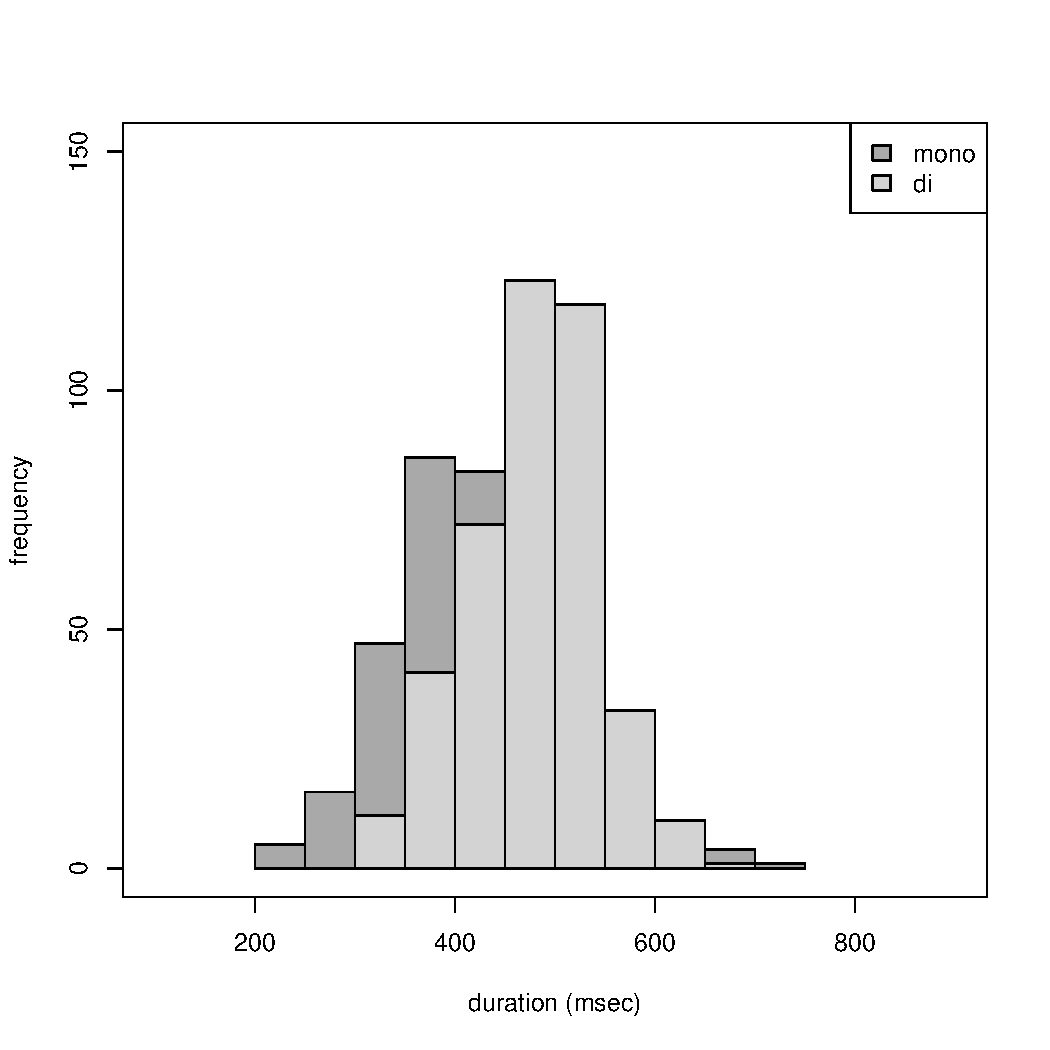
\includegraphics[width=\maxwidth]{img/word-duration-1} 

\end{knitrout}
\caption{Duration of mono- \textit{vs.} bisyllabic words.}
\end{figure}

The mean length of monosyllabic words is 434.01 msec [\textit{sd} = 88.01], while that of bisyllabic words is 478.63 msec [\textit{sd} = 63.21].

Since I am looking at the duration of the normalised modal voicing of the vocalic gesture, we should first check if there is a significant difference in length of modal voicing between mono and bisyllabic words.

\begin{figure}
\begin{knitrout}
\definecolor{shadecolor}{rgb}{0.969, 0.969, 0.969}\color{fgcolor}\begin{kframe}
\begin{alltt}
\hlstd{norm_vowel_mono_density} \hlkwb{<-} \hlkwd{density}\hlstd{(mono}\hlopt{$}\hlstd{norm_vowel,} \hlkwc{na.rm} \hlstd{=} \hlnum{TRUE}\hlstd{)}
\hlstd{norm_vowel_di_density} \hlkwb{<-} \hlkwd{density}\hlstd{(bi}\hlopt{$}\hlstd{norm_vowel,} \hlkwc{na.rm} \hlstd{=} \hlnum{TRUE}\hlstd{)}

\hlstd{norm_vowel_density_x} \hlkwb{<-} \hlkwd{c}\hlstd{(norm_vowel_mono_density}\hlopt{$}\hlstd{x,}
                                  \hlstd{norm_vowel_di_density}\hlopt{$}\hlstd{x)}
\hlstd{norm_vowel_density_y} \hlkwb{<-} \hlkwd{c}\hlstd{(norm_vowel_mono_density}\hlopt{$}\hlstd{y,}
                                  \hlstd{norm_vowel_di_density}\hlopt{$}\hlstd{y)}

\hlstd{x.limits} \hlkwb{<-} \hlkwd{range}\hlstd{(norm_vowel_density_x)}
\hlstd{y.limits} \hlkwb{<-} \hlkwd{range}\hlstd{(norm_vowel_density_y)}

\hlkwd{plot}\hlstd{(}
\hlkwd{c}\hlstd{(),} \hlkwd{c}\hlstd{(),}
\hlkwc{xlim} \hlstd{= x.limits,}
\hlkwc{ylim} \hlstd{= y.limits,}
\hlkwc{xlab} \hlstd{=} \hlstr{"duration (s)"}\hlstd{,} \hlkwc{ylab} \hlstd{=} \hlstr{"density"}
\hlstd{)}

\hlkwd{lines}\hlstd{(norm_vowel_mono_density,} \hlkwc{lw} \hlstd{=} \hlnum{1}\hlstd{)}
\hlkwd{lines}\hlstd{(norm_vowel_di_density,} \hlkwc{lw} \hlstd{=} \hlnum{1}\hlstd{,} \hlkwc{lty} \hlstd{=} \hlnum{2}\hlstd{)}

\hlkwd{legend}\hlstd{(}\hlstr{"topright"}\hlstd{,}
       \hlkwd{c}\hlstd{(}\hlstr{"mono"}\hlstd{,} \hlstr{"di"}\hlstd{),}
       \hlkwc{lty} \hlstd{=} \hlkwd{c}\hlstd{(}\hlnum{1}\hlstd{,}\hlnum{2}\hlstd{)}
       \hlstd{)}
\end{alltt}
\end{kframe}
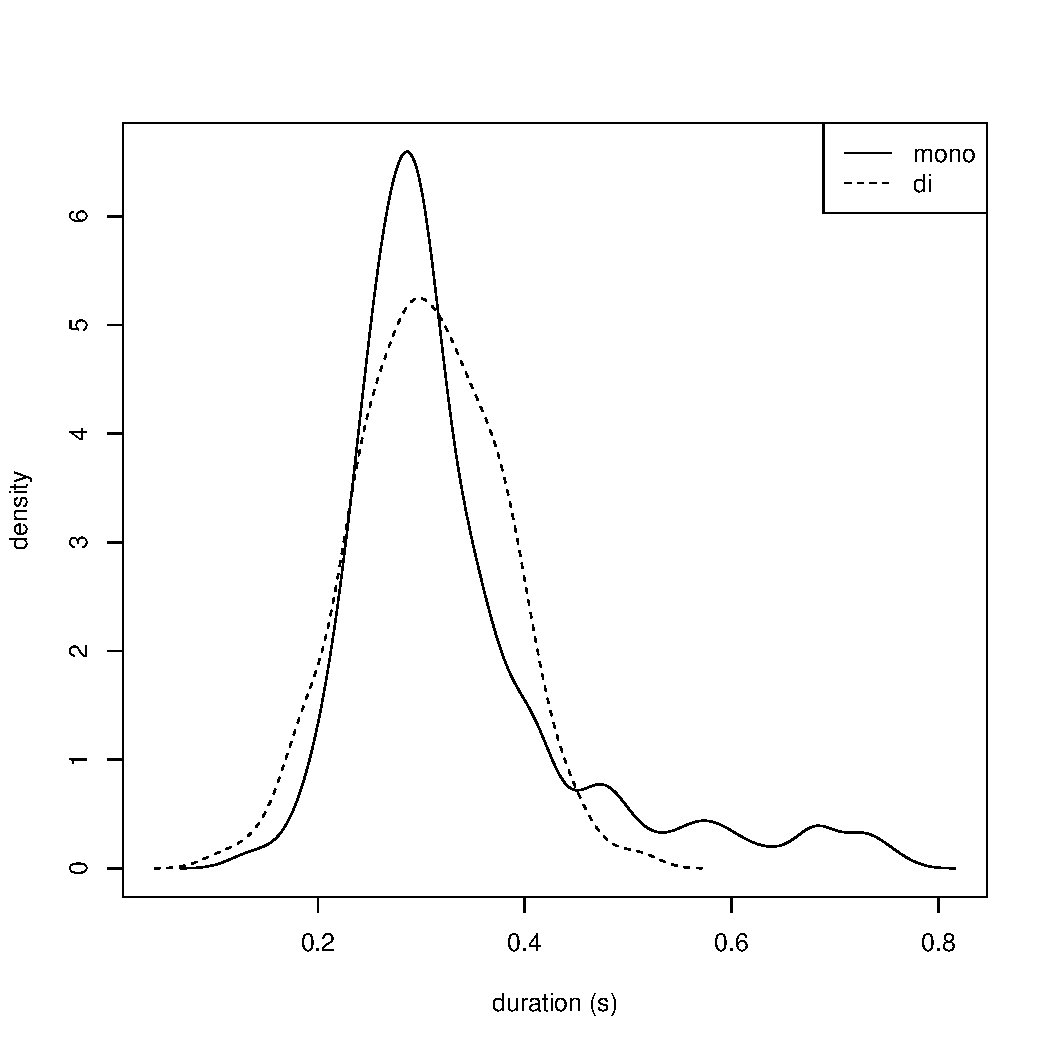
\includegraphics[width=\maxwidth]{img/mono-bi-dens-1} 

\end{knitrout}
\caption{Density plot of the duration of the voiced vocalic portion in mono- and disyllabic words.}
\end{figure}


\begin{knitrout}
\definecolor{shadecolor}{rgb}{0.969, 0.969, 0.969}\color{fgcolor}\begin{kframe}
\begin{alltt}
\hlkwd{shapiro.test}\hlstd{(mono}\hlopt{$}\hlstd{norm_vowel)}
\end{alltt}
\begin{verbatim}
## 
## 	Shapiro-Wilk normality test
## 
## data:  mono$norm_vowel
## W = 0.82764, p-value < 2.2e-16
\end{verbatim}
\begin{alltt}
\hlkwd{shapiro.test}\hlstd{(bi}\hlopt{$}\hlstd{norm_vowel)}
\end{alltt}
\begin{verbatim}
## 
## 	Shapiro-Wilk normality test
## 
## data:  bi$norm_vowel
## W = 0.99842, p-value = 0.9736
\end{verbatim}
\end{kframe}
\end{knitrout}

A Wilcox test shows that the mean length of modal voicing is significantly longer in monosyllabic words (NA) than in bisyllabic words (NA).
Subsequent tests will be performed for monosyllabic and bisyllabic words separately.

\begin{knitrout}
\definecolor{shadecolor}{rgb}{0.969, 0.969, 0.969}\color{fgcolor}\begin{kframe}
\begin{alltt}
\hlkwd{wilcox.test}\hlstd{(mono}\hlopt{$}\hlstd{norm_vowel, bi}\hlopt{$}\hlstd{norm_vowel)}
\end{alltt}
\begin{verbatim}
## 
## 	Wilcoxon rank sum test with continuity correction
## 
## data:  mono$norm_vowel and bi$norm_vowel
## W = 82451, p-value = 0.309
## alternative hypothesis: true location shift is not equal to 0
\end{verbatim}
\end{kframe}
\end{knitrout}

\section{Monosyllabic words}

\subsection{Stops}

We can now have a look at monosyllabic words, starting from CVCC words (ending in a geminate stop).
These words start with either an aspirated, a non-aspirated or a sonorant consonant.

\begin{knitrout}
\definecolor{shadecolor}{rgb}{0.969, 0.969, 0.969}\color{fgcolor}\begin{kframe}
\begin{alltt}
\hlstd{mono_stop} \hlkwb{<-} \hlkwd{subset}\hlstd{(mono, manner} \hlopt{==} \hlstr{"stop"}\hlstd{)}

\hlstd{di_stop} \hlkwb{<-} \hlkwd{subset}\hlstd{(bi, manner} \hlopt{==} \hlstr{"stop"}\hlstd{)}

\hlstd{mono_stop_asp} \hlkwb{<-} \hlstd{mono_stop}\hlopt{$}\hlstd{norm_vowel[mono_stop}\hlopt{$}\hlstd{asp} \hlopt{==} \hlstr{"yes"}\hlstd{]}
\hlstd{mono_stop_nasp} \hlkwb{<-} \hlstd{mono_stop}\hlopt{$}\hlstd{norm_vowel[mono_stop}\hlopt{$}\hlstd{asp} \hlopt{==} \hlstr{"no"}\hlstd{]}

\hlstd{norm_vowel_asp_density} \hlkwb{<-} \hlkwd{density}\hlstd{(mono_stop_asp)}
\hlstd{norm_vowel_nasp_density} \hlkwb{<-} \hlkwd{density}\hlstd{(mono_stop_nasp)}

\hlstd{norm_vowel_density_x} \hlkwb{<-} \hlkwd{c}\hlstd{(norm_vowel_asp_density}\hlopt{$}\hlstd{x,}
                                  \hlstd{norm_vowel_nasp_density}\hlopt{$}\hlstd{x)}
\hlstd{norm_vowel_density_y} \hlkwb{<-} \hlkwd{c}\hlstd{(norm_vowel_asp_density}\hlopt{$}\hlstd{y,}
                                  \hlstd{norm_vowel_nasp_density}\hlopt{$}\hlstd{y)}

\hlstd{x.limits} \hlkwb{<-} \hlkwd{range}\hlstd{(norm_vowel_density_x)}
\hlstd{y.limits} \hlkwb{<-} \hlkwd{range}\hlstd{(norm_vowel_density_y)}

\hlkwd{plot}\hlstd{(}
\hlkwd{c}\hlstd{(),} \hlkwd{c}\hlstd{(),}
\hlkwc{xlim} \hlstd{= x.limits,}
\hlkwc{ylim} \hlstd{= y.limits,}
\hlkwc{xlab} \hlstd{=} \hlstr{"duration (s)"}\hlstd{,} \hlkwc{ylab} \hlstd{=} \hlstr{"density"}
\hlstd{)}

\hlkwd{lines}\hlstd{(norm_vowel_asp_density,} \hlkwc{lw} \hlstd{=} \hlnum{1}\hlstd{,} \hlkwc{col} \hlstd{=} \hlstr{"blue"}\hlstd{)}
\hlkwd{lines}\hlstd{(norm_vowel_nasp_density,} \hlkwc{lw} \hlstd{=} \hlnum{1}\hlstd{,} \hlkwc{col} \hlstd{=} \hlstr{"red"}\hlstd{)}
\end{alltt}
\end{kframe}
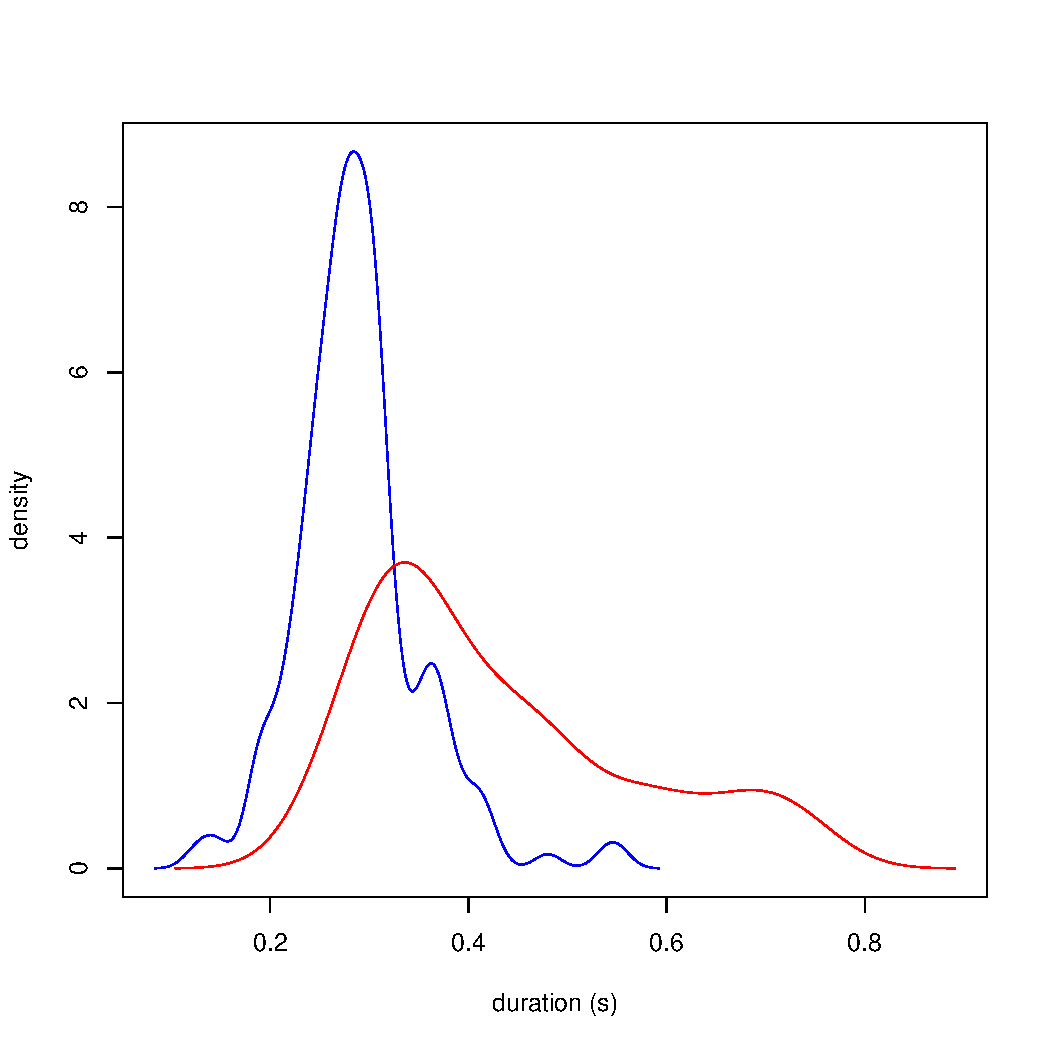
\includegraphics[width=\maxwidth]{img/mono-stop-dens-1} 

\end{knitrout}

\begin{knitrout}
\definecolor{shadecolor}{rgb}{0.969, 0.969, 0.969}\color{fgcolor}\begin{kframe}
\begin{alltt}
\hlkwd{shapiro.test}\hlstd{(mono_stop_asp)}
\end{alltt}
\begin{verbatim}
## 
## 	Shapiro-Wilk normality test
## 
## data:  mono_stop_asp
## W = 0.94276, p-value = 2.565e-06
\end{verbatim}
\begin{alltt}
\hlkwd{shapiro.test}\hlstd{(mono_stop_nasp)}
\end{alltt}
\begin{verbatim}
## 
## 	Shapiro-Wilk normality test
## 
## data:  mono_stop_nasp
## W = 0.90257, p-value = 1.673e-07
\end{verbatim}
\end{kframe}
\end{knitrout}

Since the distributions of the duration of modal voicing in the two conditions (pre-aspirated and non-aspirated) are significantly different from the normal distribution, we should perform a Wilcoxon test.
According to the test, the mean duration of modal voicing in words ending with a pre-aspirated stop is significantly shorter (0.29 seconds) than in words ending with a non-aspirated stop (0.43 seconds).

\begin{knitrout}
\definecolor{shadecolor}{rgb}{0.969, 0.969, 0.969}\color{fgcolor}\begin{kframe}
\begin{alltt}
\hlkwd{boxplot}\hlstd{(norm_vowel} \hlopt{~} \hlstd{asp,}
        \hlkwc{data} \hlstd{= mono_stop,}
        \hlkwc{names} \hlstd{=} \hlkwd{c}\hlstd{(}\hlstr{"non-asp"}\hlstd{,} \hlstr{"asp"}\hlstd{),}
        \hlkwc{ylab} \hlstd{=} \hlstr{"duration (msec)"}\hlstd{,}
        \hlkwc{main} \hlstd{=} \hlstr{"Duration (in seconds) of modal voicing in CVCC words"}
        \hlstd{)}
\end{alltt}
\end{kframe}
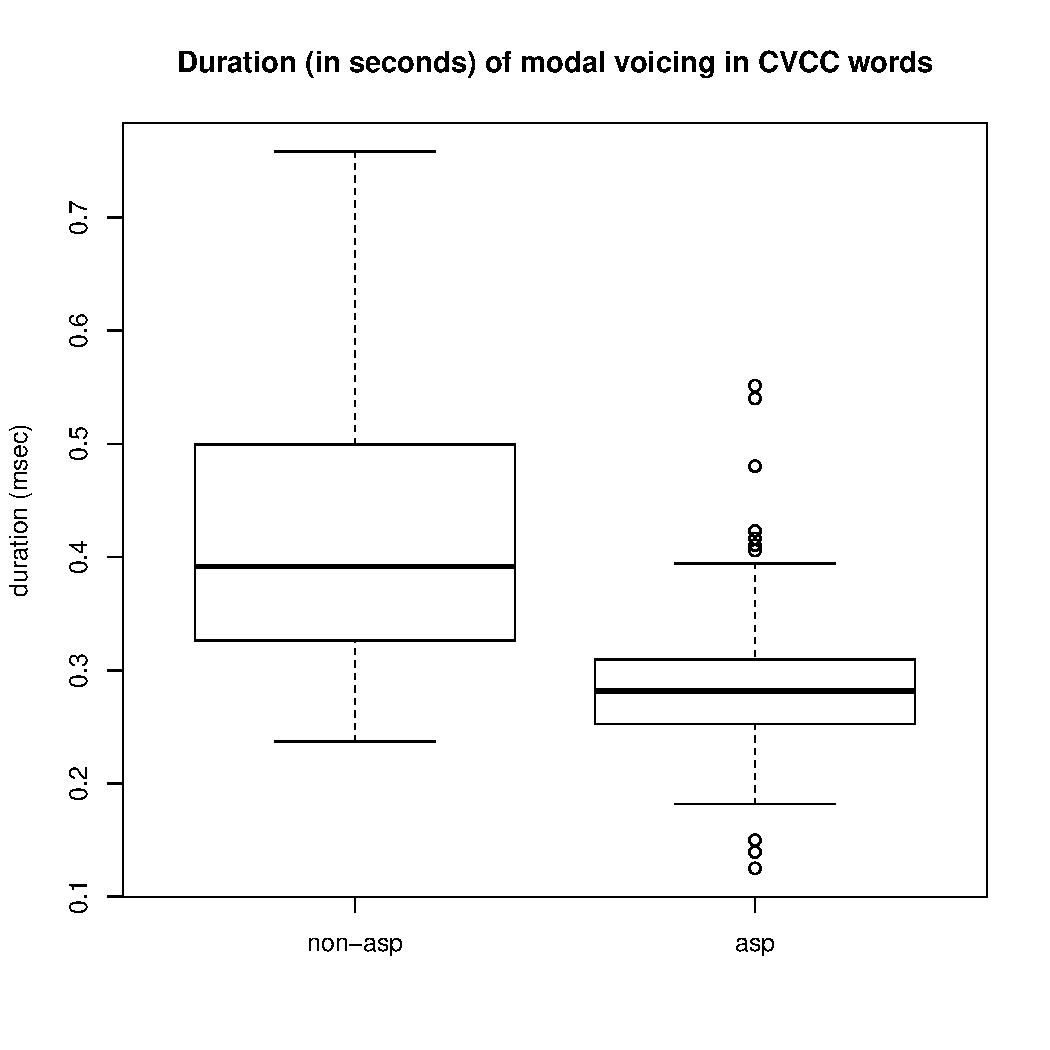
\includegraphics[width=\maxwidth]{img/mono-stop-box-1} 
\begin{kframe}\begin{alltt}
\hlkwd{wilcox.test}\hlstd{(norm_vowel} \hlopt{~} \hlstd{asp,} \hlkwc{data} \hlstd{= mono_stop)}
\end{alltt}
\begin{verbatim}
## 
## 	Wilcoxon rank sum test with continuity correction
## 
## data:  norm_vowel by asp
## W = 18010, p-value < 2.2e-16
## alternative hypothesis: true location shift is not equal to 0
\end{verbatim}
\end{kframe}
\end{knitrout}

\subsection{Nasals}

\begin{knitrout}
\definecolor{shadecolor}{rgb}{0.969, 0.969, 0.969}\color{fgcolor}\begin{kframe}
\begin{alltt}
\hlstd{mono_nas} \hlkwb{<-} \hlkwd{subset}\hlstd{(mono, manner} \hlopt{==} \hlstr{"nasal"}\hlstd{)}
\end{alltt}
\end{kframe}
\end{knitrout}

\begin{knitrout}
\definecolor{shadecolor}{rgb}{0.969, 0.969, 0.969}\color{fgcolor}\begin{kframe}
\begin{alltt}
\hlstd{mono_nas_asp} \hlkwb{<-} \hlstd{mono_nas}\hlopt{$}\hlstd{norm_vowel[mono_nas}\hlopt{$}\hlstd{asp} \hlopt{==} \hlstr{"yes"}\hlstd{]}
\hlstd{mono_nas_nasp} \hlkwb{<-} \hlstd{mono_nas}\hlopt{$}\hlstd{norm_vowel[mono_nas}\hlopt{$}\hlstd{asp} \hlopt{==} \hlstr{"no"}\hlstd{]}

\hlstd{norm_vowel_asp_density} \hlkwb{<-} \hlkwd{density}\hlstd{(mono_nas_asp)}
\hlstd{norm_vowel_nasp_density} \hlkwb{<-} \hlkwd{density}\hlstd{(mono_nas_nasp)}

\hlstd{norm_vowel_density_x} \hlkwb{<-} \hlkwd{c}\hlstd{(norm_vowel_asp_density}\hlopt{$}\hlstd{x,}
                                  \hlstd{norm_vowel_nasp_density}\hlopt{$}\hlstd{x)}
\hlstd{norm_vowel_density_y} \hlkwb{<-} \hlkwd{c}\hlstd{(norm_vowel_asp_density}\hlopt{$}\hlstd{y,}
                                  \hlstd{norm_vowel_nasp_density}\hlopt{$}\hlstd{y)}

\hlstd{x.limits} \hlkwb{<-} \hlkwd{range}\hlstd{(norm_vowel_density_x)}
\hlstd{y.limits} \hlkwb{<-} \hlkwd{range}\hlstd{(norm_vowel_density_y)}

\hlkwd{plot}\hlstd{(}
\hlkwd{c}\hlstd{(),} \hlkwd{c}\hlstd{(),}
\hlkwc{xlim} \hlstd{= x.limits,}
\hlkwc{ylim} \hlstd{= y.limits,}
\hlkwc{xlab} \hlstd{=} \hlstr{"duration (s)"}\hlstd{,} \hlkwc{ylab} \hlstd{=} \hlstr{"density"}
\hlstd{)}

\hlkwd{lines}\hlstd{(norm_vowel_asp_density,} \hlkwc{lw} \hlstd{=} \hlnum{1}\hlstd{,} \hlkwc{col} \hlstd{=} \hlstr{"blue"}\hlstd{)}
\hlkwd{lines}\hlstd{(norm_vowel_nasp_density,} \hlkwc{lw} \hlstd{=} \hlnum{1}\hlstd{,} \hlkwc{col} \hlstd{=} \hlstr{"red"}\hlstd{)}
\end{alltt}
\end{kframe}
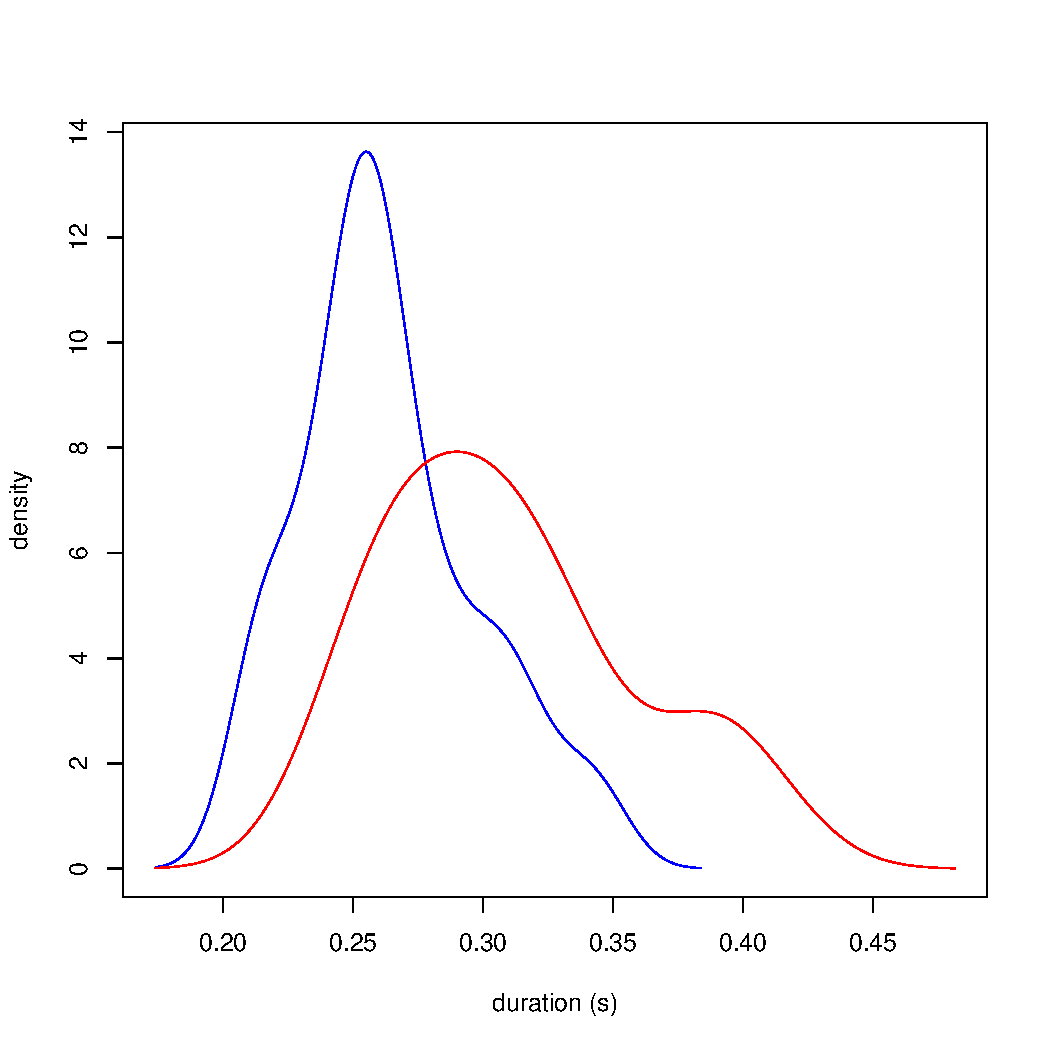
\includegraphics[width=\maxwidth]{img/mono-nas-dens-1} 

\end{knitrout}

\begin{knitrout}
\definecolor{shadecolor}{rgb}{0.969, 0.969, 0.969}\color{fgcolor}\begin{kframe}
\begin{alltt}
\hlkwd{boxplot}\hlstd{(norm_vowel} \hlopt{~} \hlstd{asp,}
        \hlkwc{data} \hlstd{= mono_nas,}
        \hlkwc{names} \hlstd{=} \hlkwd{c}\hlstd{(}\hlstr{"non-asp"}\hlstd{,} \hlstr{"asp"}\hlstd{),}
        \hlkwc{ylab} \hlstd{=} \hlstr{"duration (s)"}\hlstd{,}
        \hlkwc{main} \hlstd{=} \hlstr{"Duration (in seconds) of modal voicing in CVNC words"}
        \hlstd{)}
\end{alltt}
\end{kframe}
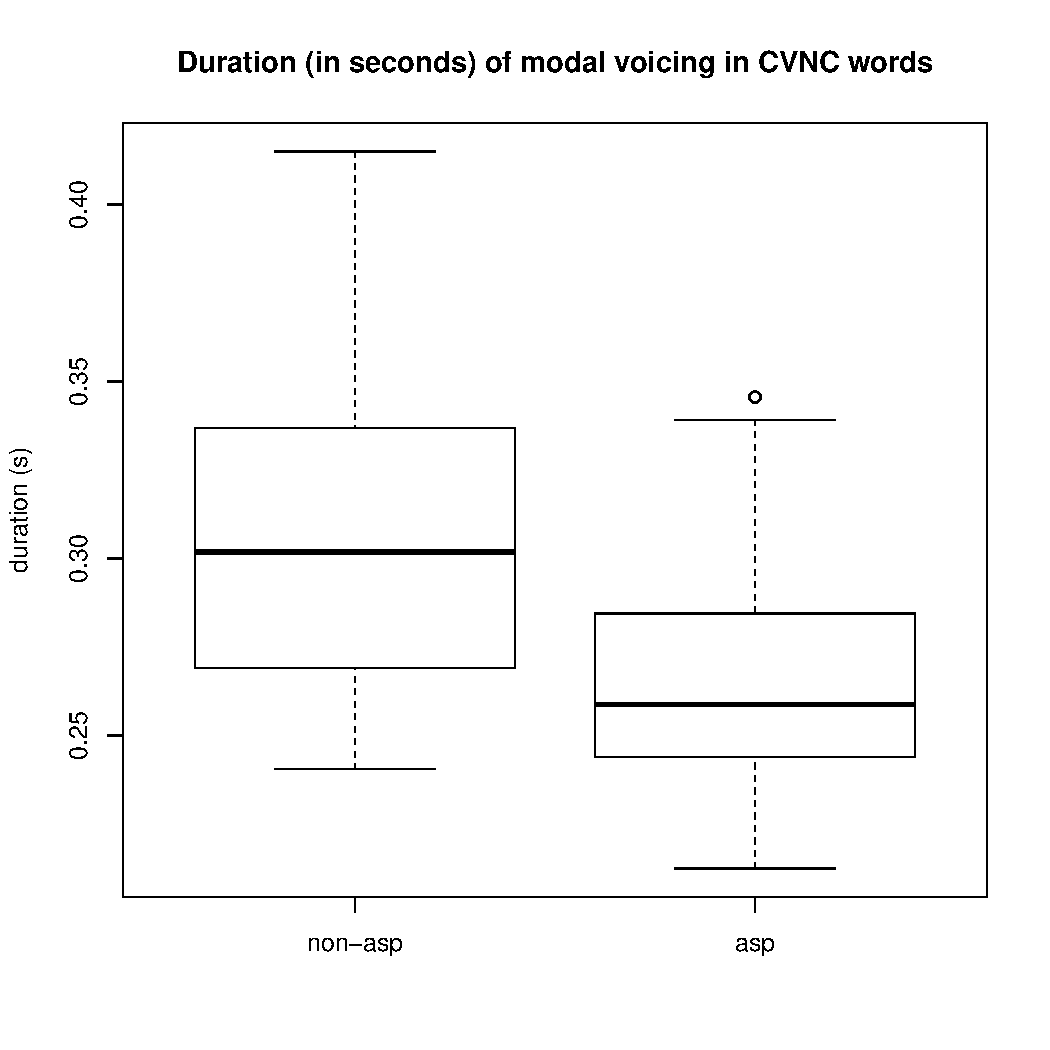
\includegraphics[width=\maxwidth]{img/mono-nas-box-1} 

\end{knitrout}

\begin{knitrout}
\definecolor{shadecolor}{rgb}{0.969, 0.969, 0.969}\color{fgcolor}\begin{kframe}
\begin{alltt}
\hlkwd{shapiro.test}\hlstd{(mono_nas_asp)}
\end{alltt}
\begin{verbatim}
## 
## 	Shapiro-Wilk normality test
## 
## data:  mono_nas_asp
## W = 0.94983, p-value = 0.0879
\end{verbatim}
\begin{alltt}
\hlkwd{shapiro.test}\hlstd{(mono_nas_nasp)}
\end{alltt}
\begin{verbatim}
## 
## 	Shapiro-Wilk normality test
## 
## data:  mono_nas_nasp
## W = 0.94149, p-value = 0.1097
\end{verbatim}
\begin{alltt}
\hlkwd{t.test}\hlstd{(norm_vowel} \hlopt{~} \hlstd{asp,} \hlkwc{data} \hlstd{= mono_nas)}
\end{alltt}
\begin{verbatim}
## 
## 	Welch Two Sample t-test
## 
## data:  norm_vowel by asp
## t = 4.3754, df = 48.072, p-value = 6.497e-05
## alternative hypothesis: true difference in means is not equal to 0
## 95 percent confidence interval:
##  0.02495378 0.06738528
## sample estimates:
##  mean in group no mean in group yes 
##         0.3098634         0.2636939
\end{verbatim}
\end{kframe}
\end{knitrout}

According to a two-sample \textit{t}-test, the duration of modal voicing in words ending with an N̥C cluster (0.26 seconds) is shorter than in words ending with an NC cluster (0.31 seconds).

\subsection{Laterals}

\begin{knitrout}
\definecolor{shadecolor}{rgb}{0.969, 0.969, 0.969}\color{fgcolor}\begin{kframe}
\begin{alltt}
\hlstd{mono_lat} \hlkwb{<-} \hlkwd{subset}\hlstd{(mono, manner} \hlopt{==} \hlstr{"lateral"}\hlstd{)}
\end{alltt}
\end{kframe}
\end{knitrout}

\begin{knitrout}
\definecolor{shadecolor}{rgb}{0.969, 0.969, 0.969}\color{fgcolor}\begin{kframe}
\begin{alltt}
\hlstd{mono_lat_asp} \hlkwb{<-} \hlstd{mono_lat}\hlopt{$}\hlstd{norm_vowel[mono_lat}\hlopt{$}\hlstd{asp} \hlopt{==} \hlstr{"yes"}\hlstd{]}
\hlstd{mono_lat_nasp} \hlkwb{<-} \hlstd{mono_lat}\hlopt{$}\hlstd{norm_vowel[mono_lat}\hlopt{$}\hlstd{asp} \hlopt{==} \hlstr{"no"}\hlstd{]}

\hlstd{norm_vowel_asp_density} \hlkwb{<-} \hlkwd{density}\hlstd{(mono_lat_asp)}
\hlstd{norm_vowel_nasp_density} \hlkwb{<-} \hlkwd{density}\hlstd{(mono_lat_nasp)}

\hlstd{norm_vowel_density_x} \hlkwb{<-} \hlkwd{c}\hlstd{(norm_vowel_asp_density}\hlopt{$}\hlstd{x,}
                                  \hlstd{norm_vowel_nasp_density}\hlopt{$}\hlstd{x)}
\hlstd{norm_vowel_density_y} \hlkwb{<-} \hlkwd{c}\hlstd{(norm_vowel_asp_density}\hlopt{$}\hlstd{y,}
                                  \hlstd{norm_vowel_nasp_density}\hlopt{$}\hlstd{y)}

\hlstd{x.limits} \hlkwb{<-} \hlkwd{range}\hlstd{(norm_vowel_density_x)}
\hlstd{y.limits} \hlkwb{<-} \hlkwd{range}\hlstd{(norm_vowel_density_y)}

\hlkwd{plot}\hlstd{(}
\hlkwd{c}\hlstd{(),} \hlkwd{c}\hlstd{(),}
\hlkwc{xlim} \hlstd{= x.limits,}
\hlkwc{ylim} \hlstd{= y.limits,}
\hlkwc{xlab} \hlstd{=} \hlstr{"duration (s)"}\hlstd{,} \hlkwc{ylab} \hlstd{=} \hlstr{"density"}
\hlstd{)}

\hlkwd{lines}\hlstd{(norm_vowel_asp_density,} \hlkwc{lw} \hlstd{=} \hlnum{1}\hlstd{,} \hlkwc{col} \hlstd{=} \hlstr{"blue"}\hlstd{)}
\hlkwd{lines}\hlstd{(norm_vowel_nasp_density,} \hlkwc{lw} \hlstd{=} \hlnum{1}\hlstd{,} \hlkwc{col} \hlstd{=} \hlstr{"red"}\hlstd{)}
\end{alltt}
\end{kframe}
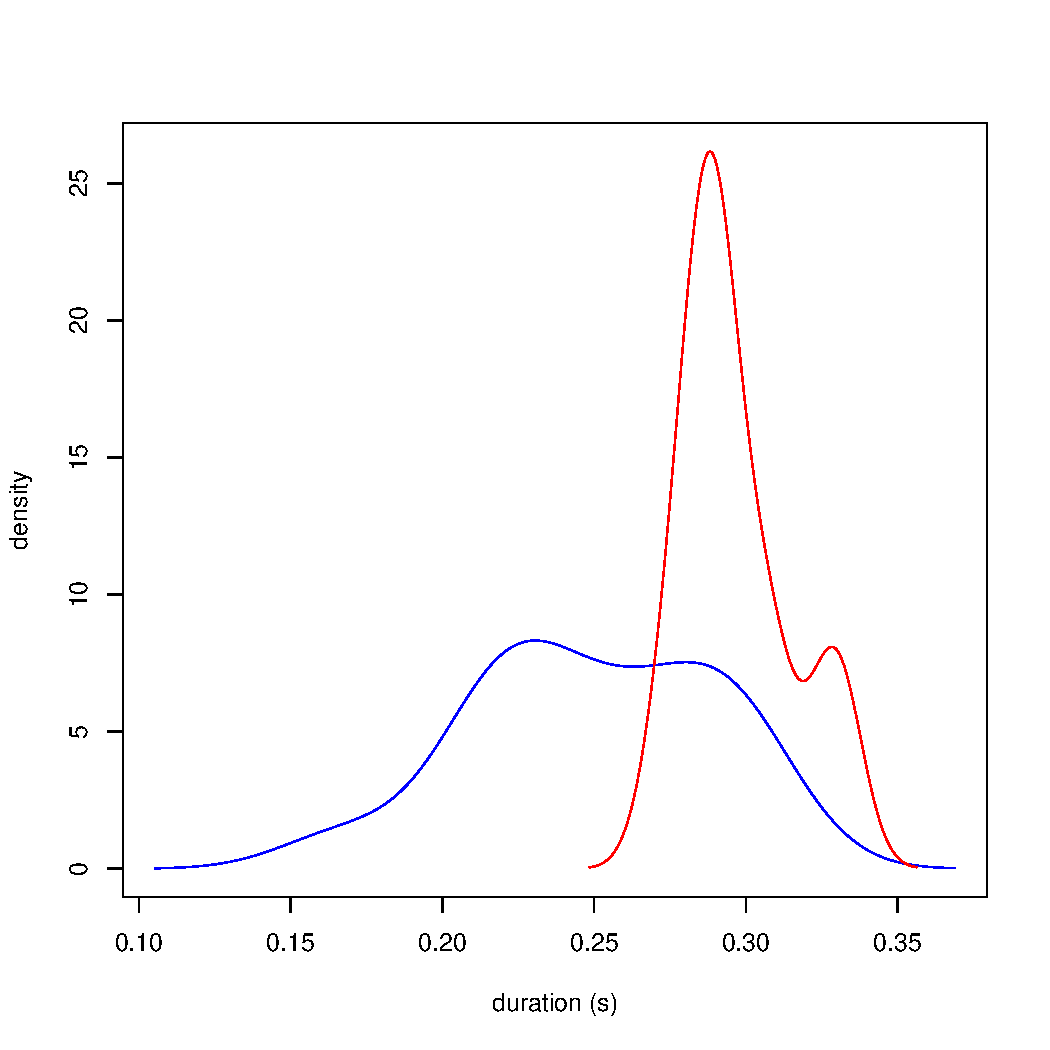
\includegraphics[width=\maxwidth]{img/mono-lat-dens-1} 

\end{knitrout}

\begin{knitrout}
\definecolor{shadecolor}{rgb}{0.969, 0.969, 0.969}\color{fgcolor}\begin{kframe}
\begin{alltt}
\hlkwd{boxplot}\hlstd{(norm_vowel} \hlopt{~} \hlstd{asp,}
        \hlkwc{data} \hlstd{= mono_lat,}
        \hlkwc{names} \hlstd{=} \hlkwd{c}\hlstd{(}\hlstr{"non-asp"}\hlstd{,} \hlstr{"asp"}\hlstd{),}
        \hlkwc{ylab} \hlstd{=} \hlstr{"duration (s)"}\hlstd{,}
        \hlkwc{main} \hlstd{=} \hlstr{"Duration (in seconds) of modal voicing in CVLC words"}
        \hlstd{)}
\end{alltt}
\end{kframe}
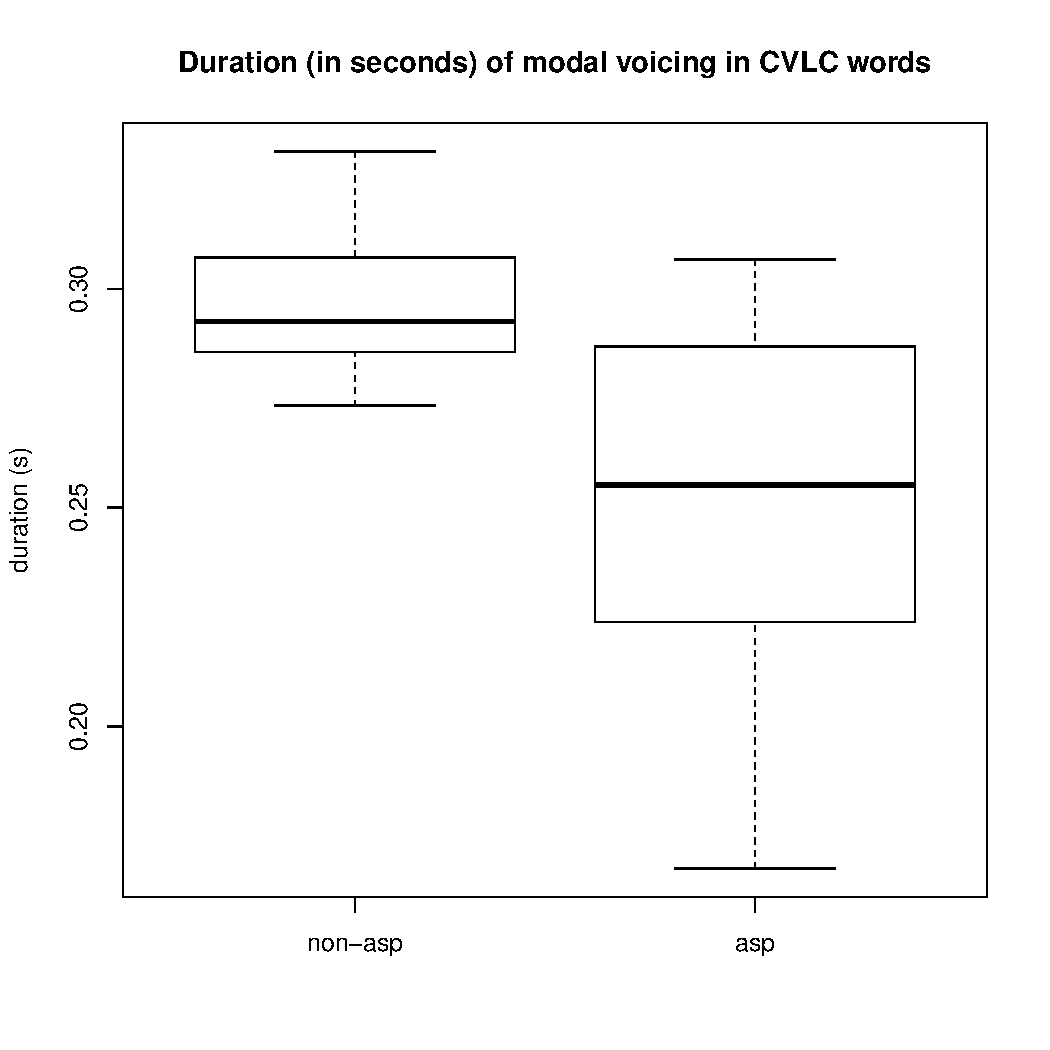
\includegraphics[width=\maxwidth]{img/mono-lat-box-1} 

\end{knitrout}

\begin{knitrout}
\definecolor{shadecolor}{rgb}{0.969, 0.969, 0.969}\color{fgcolor}\begin{kframe}
\begin{alltt}
\hlkwd{shapiro.test}\hlstd{(mono_lat_asp)}
\end{alltt}
\begin{verbatim}
## 
## 	Shapiro-Wilk normality test
## 
## data:  mono_lat_asp
## W = 0.94973, p-value = 0.5202
\end{verbatim}
\begin{alltt}
\hlkwd{shapiro.test}\hlstd{(mono_lat_nasp)}
\end{alltt}
\begin{verbatim}
## 
## 	Shapiro-Wilk normality test
## 
## data:  mono_lat_nasp
## W = 0.89635, p-value = 0.1423
\end{verbatim}
\begin{alltt}
\hlkwd{t.test}\hlstd{(norm_vowel} \hlopt{~} \hlstd{asp,} \hlkwc{data} \hlstd{= mono_lat)}
\end{alltt}
\begin{verbatim}
## 
## 	Welch Two Sample t-test
## 
## data:  norm_vowel by asp
## t = 4.1099, df = 20.43, p-value = 0.0005241
## alternative hypothesis: true difference in means is not equal to 0
## 95 percent confidence interval:
##  0.02324930 0.07104155
## sample estimates:
##  mean in group no mean in group yes 
##         0.2969002         0.2497548
\end{verbatim}
\end{kframe}
\end{knitrout}

It is good to check whether the duration of monosyllabic words is affected by the presence vs. absence of preaspiration.

\begin{knitrout}
\definecolor{shadecolor}{rgb}{0.969, 0.969, 0.969}\color{fgcolor}\begin{kframe}
\begin{alltt}
\hlkwd{boxplot}\hlstd{(dur_word} \hlopt{~} \hlstd{asp,}
        \hlkwc{data} \hlstd{= mono,}
        \hlkwc{names} \hlstd{=} \hlkwd{c}\hlstd{(}\hlstr{"non-asp"}\hlstd{,} \hlstr{"asp"}\hlstd{),}
        \hlkwc{ylab} \hlstd{=} \hlstr{"duration (s)"}\hlstd{,}
        \hlkwc{main} \hlstd{=} \hlstr{"Word duration (in seconds) depending on aspiration"}
        \hlstd{)}
\end{alltt}
\end{kframe}
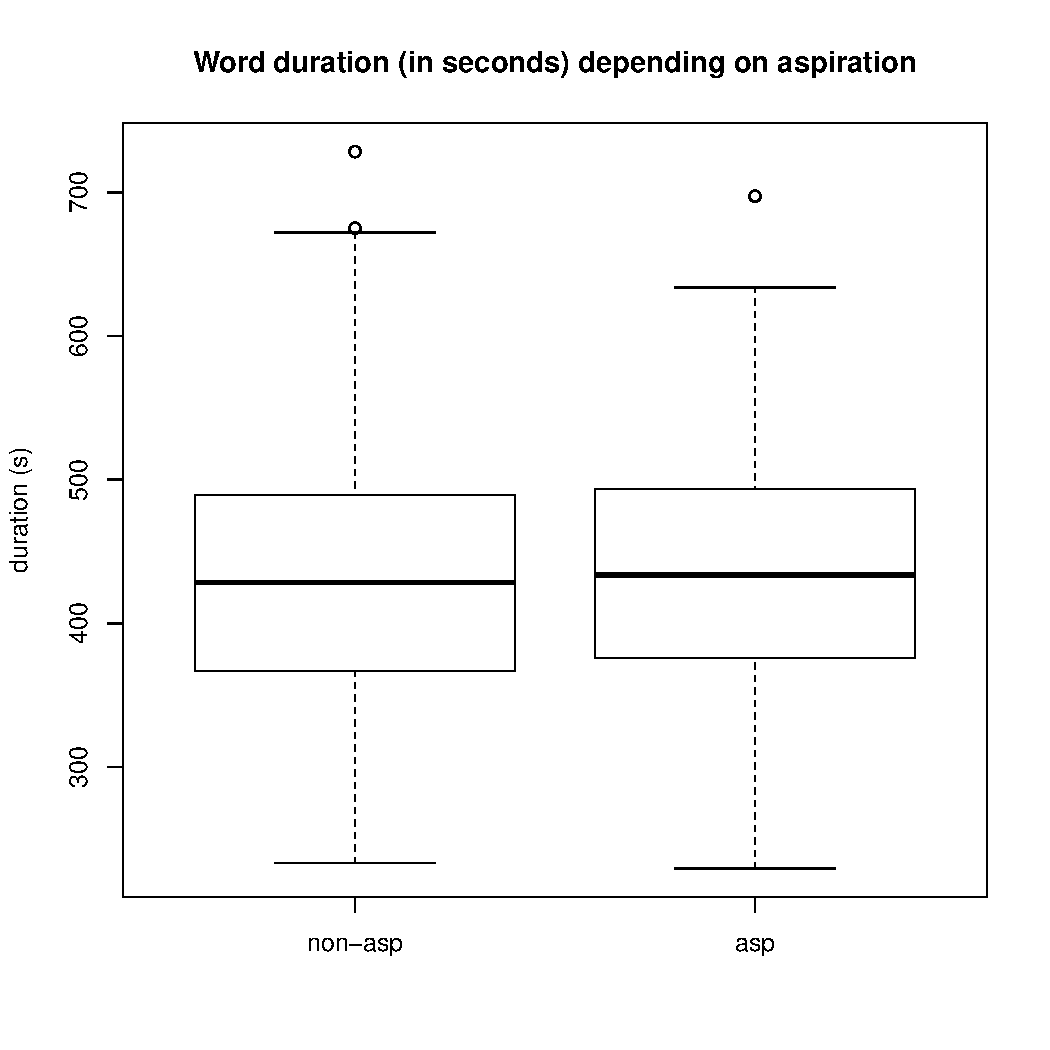
\includegraphics[width=\maxwidth]{img/mono-box-1} 

\end{knitrout}

\begin{knitrout}
\definecolor{shadecolor}{rgb}{0.969, 0.969, 0.969}\color{fgcolor}\begin{kframe}
\begin{alltt}
\hlkwd{shapiro.test}\hlstd{(mono}\hlopt{$}\hlstd{dur_word[mono}\hlopt{$}\hlstd{asp} \hlopt{==} \hlstr{"yes"}\hlstd{])}
\end{alltt}
\begin{verbatim}
## 
## 	Shapiro-Wilk normality test
## 
## data:  mono$dur_word[mono$asp == "yes"]
## W = 0.9912, p-value = 0.2007
\end{verbatim}
\begin{alltt}
\hlkwd{shapiro.test}\hlstd{(mono}\hlopt{$}\hlstd{dur_word[mono}\hlopt{$}\hlstd{asp} \hlopt{==} \hlstr{"no"}\hlstd{])}
\end{alltt}
\begin{verbatim}
## 
## 	Shapiro-Wilk normality test
## 
## data:  mono$dur_word[mono$asp == "no"]
## W = 0.98869, p-value = 0.159
\end{verbatim}
\end{kframe}
\end{knitrout}

\begin{knitrout}
\definecolor{shadecolor}{rgb}{0.969, 0.969, 0.969}\color{fgcolor}\begin{kframe}
\begin{alltt}
\hlkwd{t.test}\hlstd{(dur_word} \hlopt{~} \hlstd{asp,} \hlkwc{data} \hlstd{= mono)}
\end{alltt}
\begin{verbatim}
## 
## 	Welch Two Sample t-test
## 
## data:  dur_word by asp
## t = -0.13529, df = 351.41, p-value = 0.8925
## alternative hypothesis: true difference in means is not equal to 0
## 95 percent confidence interval:
##  -18.88264  16.45203
## sample estimates:
##  mean in group no mean in group yes 
##          433.3422          434.5575
\end{verbatim}
\end{kframe}
\end{knitrout}

According to a \textit{t}-test, the duration of monosyllabic words is not affected by the presence vs. absence of preaspiration.
Thus, the difference in the mean duration of modal voicing can't be attributed to the differences in word duration.

\section{Bisyllabic words}

\subsection{Stops}

\begin{knitrout}
\definecolor{shadecolor}{rgb}{0.969, 0.969, 0.969}\color{fgcolor}\begin{kframe}
\begin{alltt}
\hlstd{di_stop_asp} \hlkwb{<-} \hlstd{di_stop}\hlopt{$}\hlstd{norm_vowel[di_stop}\hlopt{$}\hlstd{asp} \hlopt{==} \hlstr{"yes"}\hlstd{]}
\hlstd{di_stop_nasp} \hlkwb{<-} \hlstd{di_stop}\hlopt{$}\hlstd{norm_vowel[di_stop}\hlopt{$}\hlstd{asp} \hlopt{==} \hlstr{"no"}\hlstd{]}

\hlstd{norm_vowel_asp_density} \hlkwb{<-} \hlkwd{density}\hlstd{(di_stop_asp,} \hlkwc{na.rm} \hlstd{=} \hlnum{TRUE}\hlstd{)}
\hlstd{norm_vowel_nasp_density} \hlkwb{<-} \hlkwd{density}\hlstd{(di_stop_nasp,} \hlkwc{na.rm} \hlstd{=} \hlnum{TRUE}\hlstd{)}

\hlstd{norm_vowel_density_x} \hlkwb{<-} \hlkwd{c}\hlstd{(norm_vowel_asp_density}\hlopt{$}\hlstd{x,}
                                  \hlstd{norm_vowel_nasp_density}\hlopt{$}\hlstd{x)}
\hlstd{norm_vowel_density_y} \hlkwb{<-} \hlkwd{c}\hlstd{(norm_vowel_asp_density}\hlopt{$}\hlstd{y,}
                                  \hlstd{norm_vowel_nasp_density}\hlopt{$}\hlstd{y)}

\hlstd{x.limits} \hlkwb{<-} \hlkwd{range}\hlstd{(norm_vowel_density_x)}
\hlstd{y.limits} \hlkwb{<-} \hlkwd{range}\hlstd{(norm_vowel_density_y)}

\hlkwd{plot}\hlstd{(}
\hlkwd{c}\hlstd{(),} \hlkwd{c}\hlstd{(),}
\hlkwc{xlim} \hlstd{= x.limits,}
\hlkwc{ylim} \hlstd{= y.limits,}
\hlkwc{xlab} \hlstd{=} \hlstr{"duration (s)"}\hlstd{,} \hlkwc{ylab} \hlstd{=} \hlstr{"density"}
\hlstd{)}

\hlkwd{lines}\hlstd{(norm_vowel_asp_density,} \hlkwc{lw} \hlstd{=} \hlnum{1}\hlstd{,} \hlkwc{col} \hlstd{=} \hlstr{"blue"}\hlstd{)}
\hlkwd{lines}\hlstd{(norm_vowel_nasp_density,} \hlkwc{lw} \hlstd{=} \hlnum{1}\hlstd{,} \hlkwc{col} \hlstd{=} \hlstr{"red"}\hlstd{)}
\end{alltt}
\end{kframe}
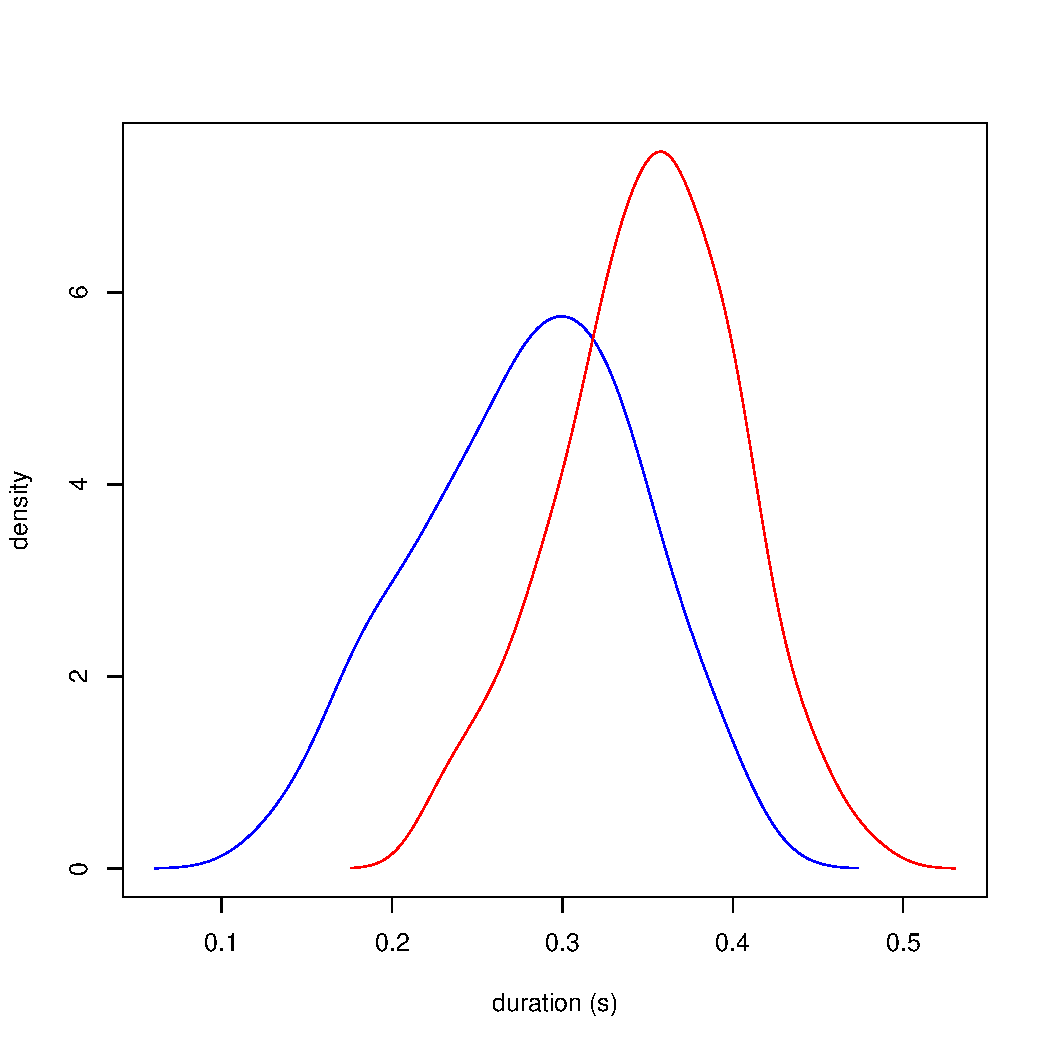
\includegraphics[width=\maxwidth]{img/bi-stop-dens-1} 

\end{knitrout}

\begin{knitrout}
\definecolor{shadecolor}{rgb}{0.969, 0.969, 0.969}\color{fgcolor}\begin{kframe}
\begin{alltt}
\hlkwd{shapiro.test}\hlstd{(di_stop_asp)}
\end{alltt}
\begin{verbatim}
## 
## 	Shapiro-Wilk normality test
## 
## data:  di_stop_asp
## W = 0.98478, p-value = 0.41
\end{verbatim}
\begin{alltt}
\hlkwd{shapiro.test}\hlstd{(di_stop_nasp)}
\end{alltt}
\begin{verbatim}
## 
## 	Shapiro-Wilk normality test
## 
## data:  di_stop_nasp
## W = 0.99166, p-value = 0.727
\end{verbatim}
\end{kframe}
\end{knitrout}

\begin{knitrout}
\definecolor{shadecolor}{rgb}{0.969, 0.969, 0.969}\color{fgcolor}\begin{kframe}
\begin{alltt}
\hlkwd{boxplot}\hlstd{(norm_vowel} \hlopt{~} \hlstd{asp,}
        \hlkwc{data} \hlstd{= di_stop,}
        \hlkwc{names} \hlstd{=} \hlkwd{c}\hlstd{(}\hlstr{"non-asp"}\hlstd{,} \hlstr{"asp"}\hlstd{),}
        \hlkwc{ylab} \hlstd{=} \hlstr{"duration (s)"}\hlstd{,}
        \hlkwc{main} \hlstd{=} \hlstr{"Duration (in seconds) of modal voicing in CVCCV words"}
        \hlstd{)}
\end{alltt}
\end{kframe}
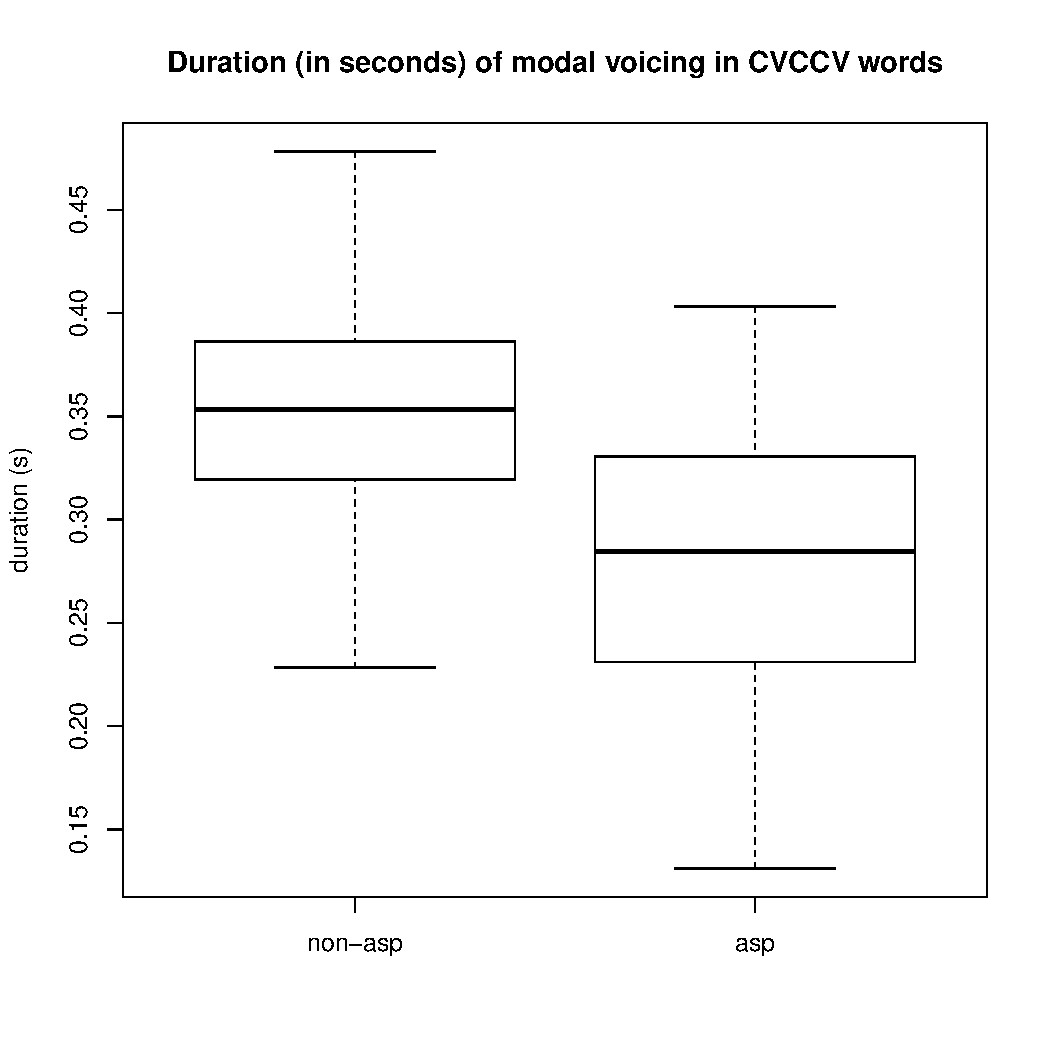
\includegraphics[width=\maxwidth]{img/bi-stop-box-1} 

\end{knitrout}

\begin{knitrout}
\definecolor{shadecolor}{rgb}{0.969, 0.969, 0.969}\color{fgcolor}\begin{kframe}
\begin{alltt}
\hlkwd{wilcox.test}\hlstd{(norm_vowel} \hlopt{~} \hlstd{asp,} \hlkwc{data} \hlstd{= mono_stop)}
\end{alltt}
\begin{verbatim}
## 
## 	Wilcoxon rank sum test with continuity correction
## 
## data:  norm_vowel by asp
## W = 18010, p-value < 2.2e-16
## alternative hypothesis: true location shift is not equal to 0
\end{verbatim}
\end{kframe}
\end{knitrout}

\subsection{Nasals}

\begin{knitrout}
\definecolor{shadecolor}{rgb}{0.969, 0.969, 0.969}\color{fgcolor}\begin{kframe}
\begin{alltt}
\hlstd{di_nas} \hlkwb{<-} \hlkwd{subset}\hlstd{(bi, manner} \hlopt{==} \hlstr{"nasal"}\hlstd{)}
\end{alltt}
\end{kframe}
\end{knitrout}

\begin{knitrout}
\definecolor{shadecolor}{rgb}{0.969, 0.969, 0.969}\color{fgcolor}\begin{kframe}
\begin{alltt}
\hlstd{di_nas_asp} \hlkwb{<-} \hlstd{di_nas}\hlopt{$}\hlstd{norm_vowel[di_nas}\hlopt{$}\hlstd{asp} \hlopt{==} \hlstr{"yes"}\hlstd{]}
\hlstd{di_nas_nasp} \hlkwb{<-} \hlstd{di_nas}\hlopt{$}\hlstd{norm_vowel[di_nas}\hlopt{$}\hlstd{asp} \hlopt{==} \hlstr{"no"}\hlstd{]}

\hlstd{norm_vowel_asp_density} \hlkwb{<-} \hlkwd{density}\hlstd{(di_nas_asp)}
\hlstd{norm_vowel_nasp_density} \hlkwb{<-} \hlkwd{density}\hlstd{(di_nas_nasp)}

\hlstd{norm_vowel_density_x} \hlkwb{<-} \hlkwd{c}\hlstd{(norm_vowel_asp_density}\hlopt{$}\hlstd{x,}
                                  \hlstd{norm_vowel_nasp_density}\hlopt{$}\hlstd{x)}
\hlstd{norm_vowel_density_y} \hlkwb{<-} \hlkwd{c}\hlstd{(norm_vowel_asp_density}\hlopt{$}\hlstd{y,}
                                  \hlstd{norm_vowel_nasp_density}\hlopt{$}\hlstd{y)}

\hlstd{x.limits} \hlkwb{<-} \hlkwd{range}\hlstd{(norm_vowel_density_x)}
\hlstd{y.limits} \hlkwb{<-} \hlkwd{range}\hlstd{(norm_vowel_density_y)}

\hlkwd{plot}\hlstd{(}
\hlkwd{c}\hlstd{(),} \hlkwd{c}\hlstd{(),}
\hlkwc{xlim} \hlstd{= x.limits,}
\hlkwc{ylim} \hlstd{= y.limits,}
\hlkwc{xlab} \hlstd{=} \hlstr{"duration (s)"}\hlstd{,} \hlkwc{ylab} \hlstd{=} \hlstr{"density"}
\hlstd{)}

\hlkwd{lines}\hlstd{(norm_vowel_asp_density,} \hlkwc{lw} \hlstd{=} \hlnum{1}\hlstd{,} \hlkwc{col} \hlstd{=} \hlstr{"blue"}\hlstd{)}
\hlkwd{lines}\hlstd{(norm_vowel_nasp_density,} \hlkwc{lw} \hlstd{=} \hlnum{1}\hlstd{,} \hlkwc{col} \hlstd{=} \hlstr{"red"}\hlstd{)}
\end{alltt}
\end{kframe}
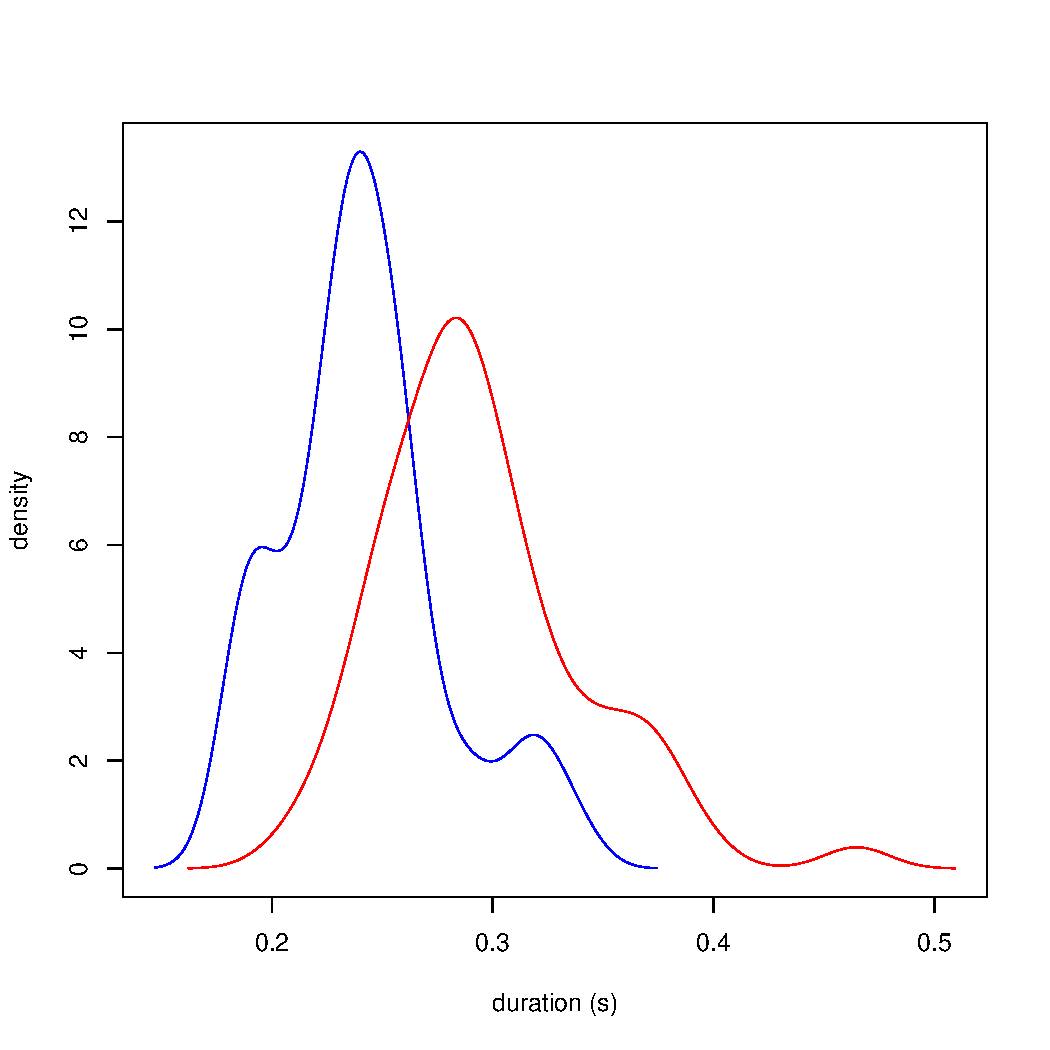
\includegraphics[width=\maxwidth]{img/bi-nas-dens-1} 

\end{knitrout}

\begin{knitrout}
\definecolor{shadecolor}{rgb}{0.969, 0.969, 0.969}\color{fgcolor}\begin{kframe}
\begin{alltt}
\hlkwd{boxplot}\hlstd{(norm_vowel} \hlopt{~} \hlstd{asp,}
        \hlkwc{data} \hlstd{= di_nas,}
        \hlkwc{names} \hlstd{=} \hlkwd{c}\hlstd{(}\hlstr{"non-asp"}\hlstd{,} \hlstr{"asp"}\hlstd{),}
        \hlkwc{ylab} \hlstd{=} \hlstr{"duration (s)"}\hlstd{,}
        \hlkwc{main} \hlstd{=} \hlstr{"Duration (in seconds) of modal voicing in CVNCV words"}
        \hlstd{)}
\end{alltt}
\end{kframe}
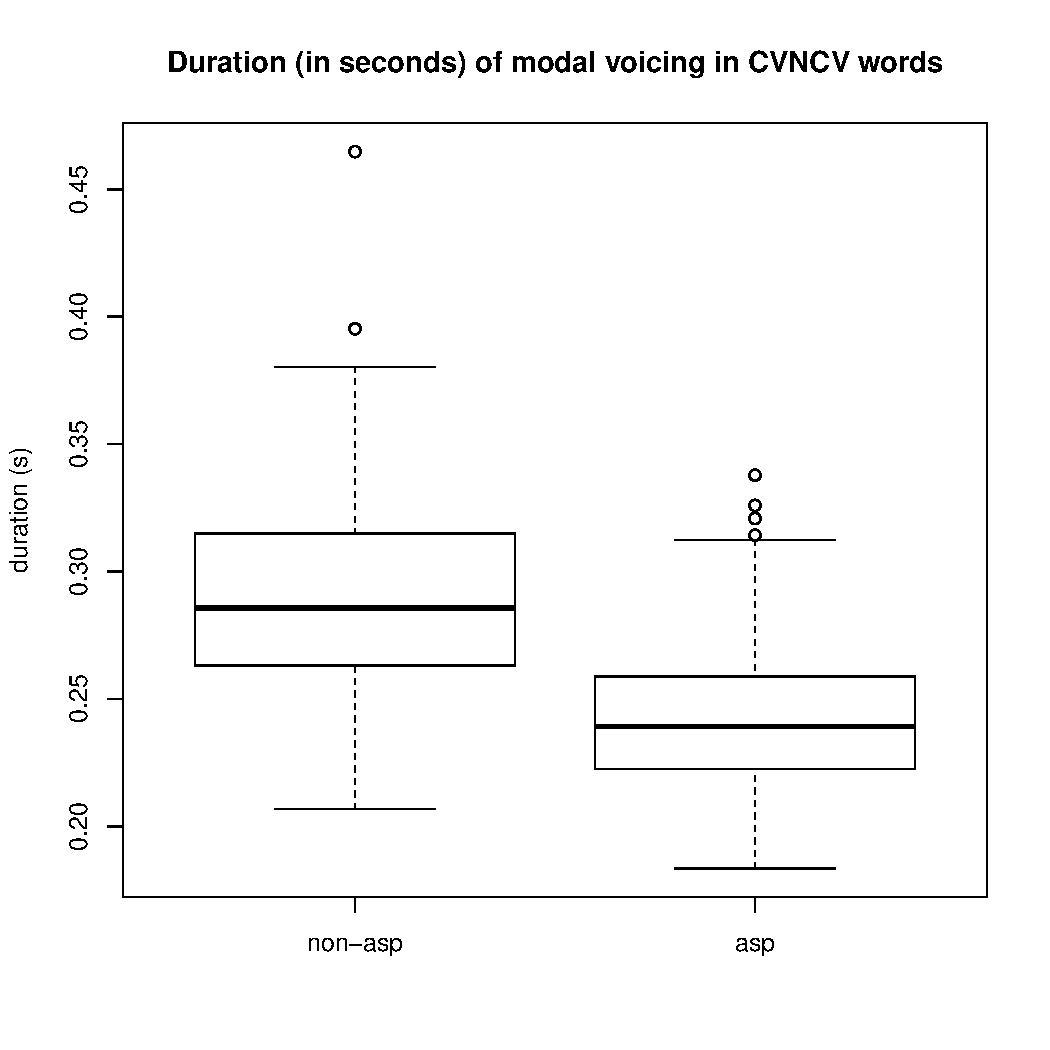
\includegraphics[width=\maxwidth]{img/bi-nas-box-1} 

\end{knitrout}

\begin{knitrout}
\definecolor{shadecolor}{rgb}{0.969, 0.969, 0.969}\color{fgcolor}\begin{kframe}
\begin{alltt}
\hlkwd{shapiro.test}\hlstd{(di_nas_asp)}
\end{alltt}
\begin{verbatim}
## 
## 	Shapiro-Wilk normality test
## 
## data:  di_nas_asp
## W = 0.9445, p-value = 0.01442
\end{verbatim}
\begin{alltt}
\hlkwd{shapiro.test}\hlstd{(di_nas_nasp)}
\end{alltt}
\begin{verbatim}
## 
## 	Shapiro-Wilk normality test
## 
## data:  di_nas_nasp
## W = 0.94685, p-value = 0.005831
\end{verbatim}
\begin{alltt}
\hlkwd{wilcox.test}\hlstd{(norm_vowel} \hlopt{~} \hlstd{asp,} \hlkwc{data} \hlstd{= di_nas)}
\end{alltt}
\begin{verbatim}
## 
## 	Wilcoxon rank sum test with continuity correction
## 
## data:  norm_vowel by asp
## W = 3052, p-value = 3.721e-10
## alternative hypothesis: true location shift is not equal to 0
\end{verbatim}
\end{kframe}
\end{knitrout}

\subsection{Laterals}

\begin{knitrout}
\definecolor{shadecolor}{rgb}{0.969, 0.969, 0.969}\color{fgcolor}\begin{kframe}
\begin{alltt}
\hlstd{di_lat} \hlkwb{<-} \hlkwd{subset}\hlstd{(bi, manner} \hlopt{==} \hlstr{"lateral"}\hlstd{)}
\end{alltt}
\end{kframe}
\end{knitrout}

\begin{knitrout}
\definecolor{shadecolor}{rgb}{0.969, 0.969, 0.969}\color{fgcolor}\begin{kframe}
\begin{alltt}
\hlstd{di_lat_asp} \hlkwb{<-} \hlstd{di_lat}\hlopt{$}\hlstd{norm_vowel[di_lat}\hlopt{$}\hlstd{asp} \hlopt{==} \hlstr{"yes"}\hlstd{]}
\hlstd{di_lat_nasp} \hlkwb{<-} \hlstd{di_lat}\hlopt{$}\hlstd{norm_vowel[di_lat}\hlopt{$}\hlstd{asp} \hlopt{==} \hlstr{"no"}\hlstd{]}

\hlstd{norm_vowel_asp_density} \hlkwb{<-} \hlkwd{density}\hlstd{(di_lat_asp)}
\hlstd{norm_vowel_nasp_density} \hlkwb{<-} \hlkwd{density}\hlstd{(di_lat_nasp)}

\hlstd{norm_vowel_density_x} \hlkwb{<-} \hlkwd{c}\hlstd{(norm_vowel_asp_density}\hlopt{$}\hlstd{x,}
                                  \hlstd{norm_vowel_nasp_density}\hlopt{$}\hlstd{x)}
\hlstd{norm_vowel_density_y} \hlkwb{<-} \hlkwd{c}\hlstd{(norm_vowel_asp_density}\hlopt{$}\hlstd{y,}
                                  \hlstd{norm_vowel_nasp_density}\hlopt{$}\hlstd{y)}

\hlstd{x.limits} \hlkwb{<-} \hlkwd{range}\hlstd{(norm_vowel_density_x)}
\hlstd{y.limits} \hlkwb{<-} \hlkwd{range}\hlstd{(norm_vowel_density_y)}

\hlkwd{plot}\hlstd{(}
\hlkwd{c}\hlstd{(),} \hlkwd{c}\hlstd{(),}
\hlkwc{xlim} \hlstd{= x.limits,}
\hlkwc{ylim} \hlstd{= y.limits,}
\hlkwc{xlab} \hlstd{=} \hlstr{"duration (s)"}\hlstd{,} \hlkwc{ylab} \hlstd{=} \hlstr{"density"}
\hlstd{)}

\hlkwd{lines}\hlstd{(norm_vowel_asp_density,} \hlkwc{lw} \hlstd{=} \hlnum{1}\hlstd{,} \hlkwc{col} \hlstd{=} \hlstr{"blue"}\hlstd{)}
\hlkwd{lines}\hlstd{(norm_vowel_nasp_density,} \hlkwc{lw} \hlstd{=} \hlnum{1}\hlstd{,} \hlkwc{col} \hlstd{=} \hlstr{"red"}\hlstd{)}
\end{alltt}
\end{kframe}
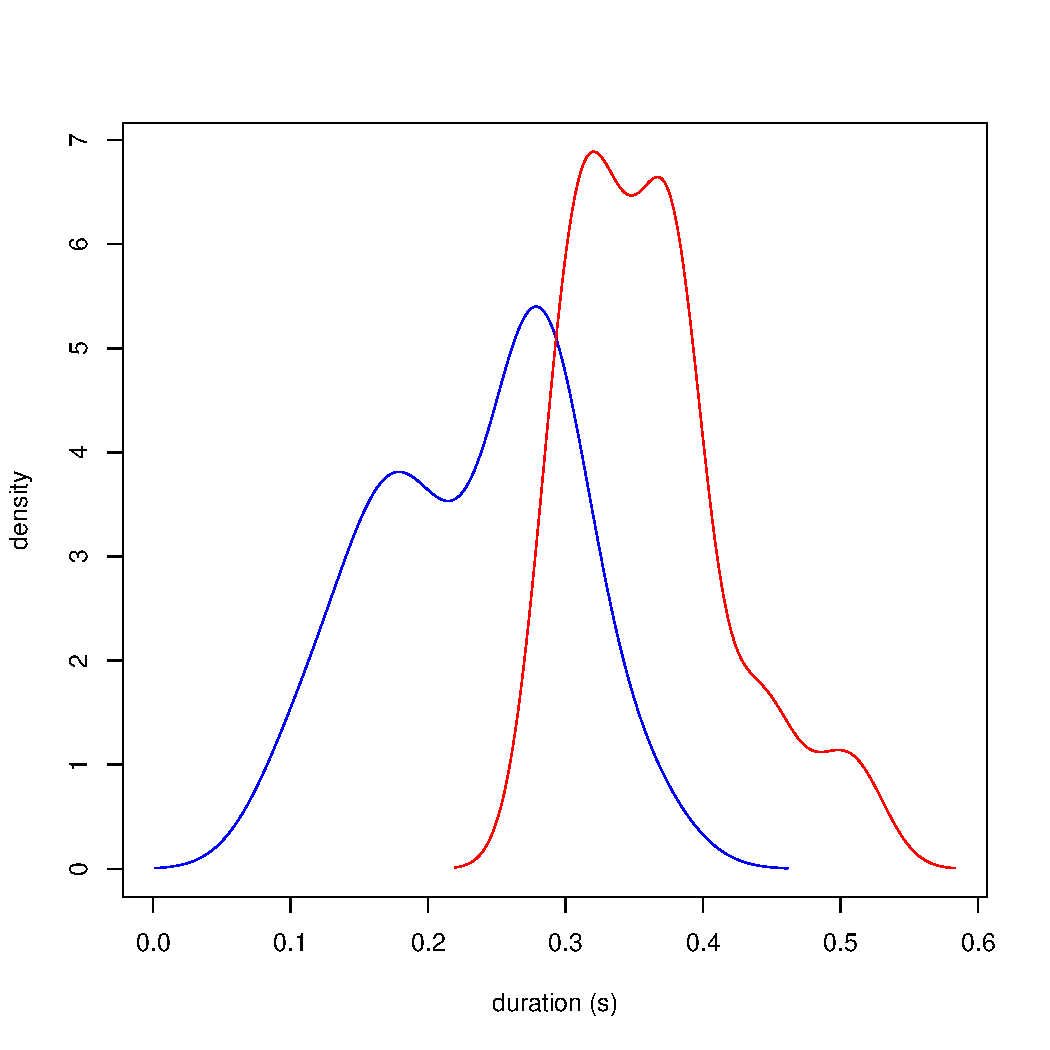
\includegraphics[width=\maxwidth]{img/bi-lat-dens-1} 

\end{knitrout}

\begin{knitrout}
\definecolor{shadecolor}{rgb}{0.969, 0.969, 0.969}\color{fgcolor}\begin{kframe}
\begin{alltt}
\hlkwd{boxplot}\hlstd{(norm_vowel} \hlopt{~} \hlstd{asp,}
        \hlkwc{data} \hlstd{= di_lat,}
        \hlkwc{names} \hlstd{=} \hlkwd{c}\hlstd{(}\hlstr{"non-asp"}\hlstd{,} \hlstr{"asp"}\hlstd{),}
        \hlkwc{ylab} \hlstd{=} \hlstr{"duration (s)"}\hlstd{,}
        \hlkwc{main} \hlstd{=} \hlstr{"Duration (in seconds) of modal voicing in CVLCV words"}
        \hlstd{)}
\end{alltt}
\end{kframe}
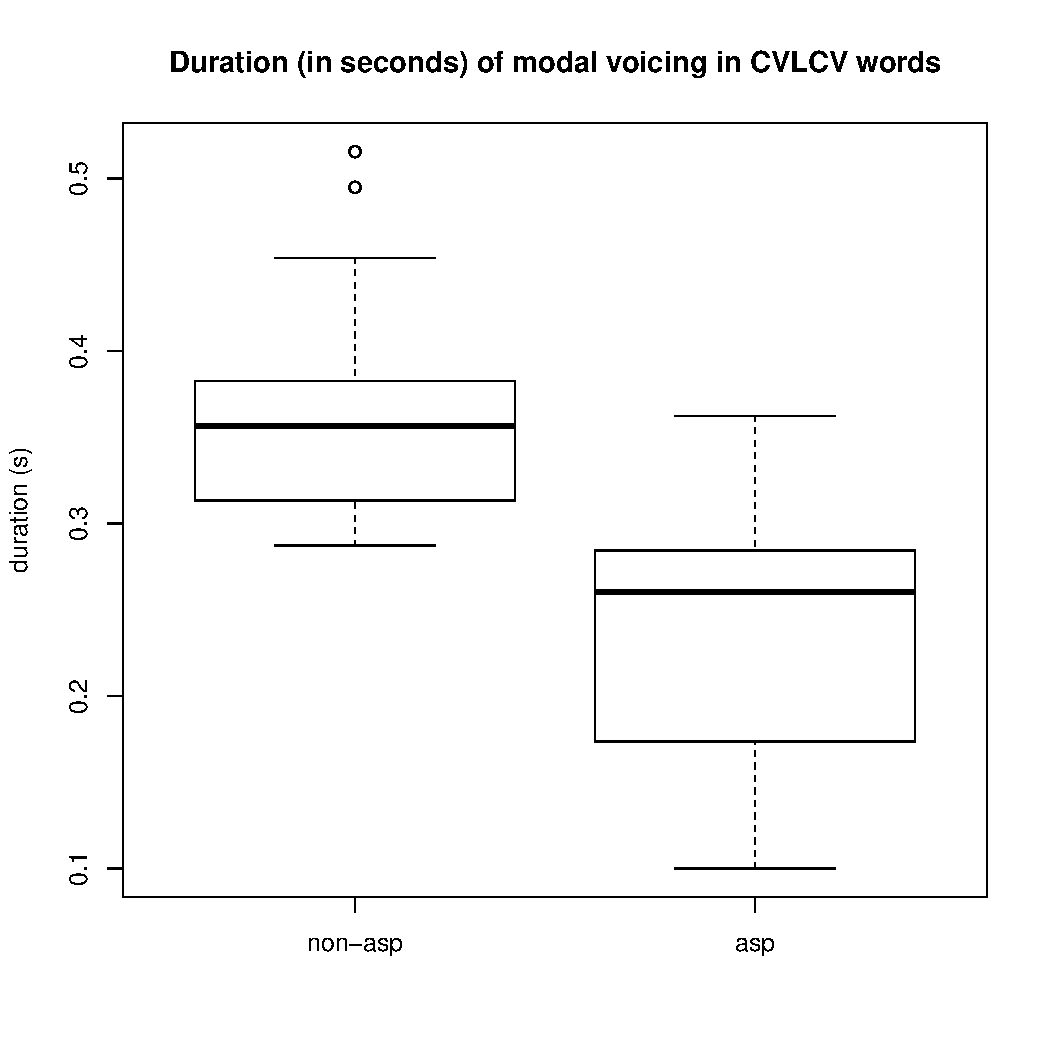
\includegraphics[width=\maxwidth]{img/bi-lat-box-1} 

\end{knitrout}

\begin{knitrout}
\definecolor{shadecolor}{rgb}{0.969, 0.969, 0.969}\color{fgcolor}\begin{kframe}
\begin{alltt}
\hlkwd{shapiro.test}\hlstd{(di_lat_asp)}
\end{alltt}
\begin{verbatim}
## 
## 	Shapiro-Wilk normality test
## 
## data:  di_lat_asp
## W = 0.95378, p-value = 0.2644
\end{verbatim}
\begin{alltt}
\hlkwd{shapiro.test}\hlstd{(di_lat_nasp)}
\end{alltt}
\begin{verbatim}
## 
## 	Shapiro-Wilk normality test
## 
## data:  di_lat_nasp
## W = 0.91062, p-value = 0.01543
\end{verbatim}
\begin{alltt}
\hlkwd{wilcox.test}\hlstd{(norm_vowel} \hlopt{~} \hlstd{asp,} \hlkwc{data} \hlstd{= di_lat)}
\end{alltt}
\begin{verbatim}
## 
## 	Wilcoxon rank sum test
## 
## data:  norm_vowel by asp
## W = 771, p-value = 2.525e-11
## alternative hypothesis: true location shift is not equal to 0
\end{verbatim}
\end{kframe}
\end{knitrout}

\subsection{Rhotics}

\begin{knitrout}
\definecolor{shadecolor}{rgb}{0.969, 0.969, 0.969}\color{fgcolor}\begin{kframe}
\begin{alltt}
\hlstd{di_rho} \hlkwb{<-} \hlkwd{subset}\hlstd{(bi, manner} \hlopt{==} \hlstr{"rhotic"}\hlstd{)}
\end{alltt}
\end{kframe}
\end{knitrout}

\begin{knitrout}
\definecolor{shadecolor}{rgb}{0.969, 0.969, 0.969}\color{fgcolor}\begin{kframe}
\begin{alltt}
\hlstd{di_rho_asp} \hlkwb{<-} \hlstd{di_rho}\hlopt{$}\hlstd{norm_vowel[di_rho}\hlopt{$}\hlstd{asp} \hlopt{==} \hlstr{"yes"}\hlstd{]}
\hlstd{di_rho_nasp} \hlkwb{<-} \hlstd{di_rho}\hlopt{$}\hlstd{norm_vowel[di_rho}\hlopt{$}\hlstd{asp} \hlopt{==} \hlstr{"no"}\hlstd{]}

\hlstd{norm_vowel_asp_density} \hlkwb{<-} \hlkwd{density}\hlstd{(di_rho_asp)}
\hlstd{norm_vowel_nasp_density} \hlkwb{<-} \hlkwd{density}\hlstd{(di_rho_nasp)}

\hlstd{norm_vowel_density_x} \hlkwb{<-} \hlkwd{c}\hlstd{(norm_vowel_asp_density}\hlopt{$}\hlstd{x,}
                                  \hlstd{norm_vowel_nasp_density}\hlopt{$}\hlstd{x)}
\hlstd{norm_vowel_density_y} \hlkwb{<-} \hlkwd{c}\hlstd{(norm_vowel_asp_density}\hlopt{$}\hlstd{y,}
                                  \hlstd{norm_vowel_nasp_density}\hlopt{$}\hlstd{y)}

\hlstd{x.limits} \hlkwb{<-} \hlkwd{range}\hlstd{(norm_vowel_density_x)}
\hlstd{y.limits} \hlkwb{<-} \hlkwd{range}\hlstd{(norm_vowel_density_y)}

\hlkwd{plot}\hlstd{(}
\hlkwd{c}\hlstd{(),} \hlkwd{c}\hlstd{(),}
\hlkwc{xlim} \hlstd{= x.limits,}
\hlkwc{ylim} \hlstd{= y.limits,}
\hlkwc{xlab} \hlstd{=} \hlstr{"duration (s)"}\hlstd{,} \hlkwc{ylab} \hlstd{=} \hlstr{"density"}
\hlstd{)}

\hlkwd{lines}\hlstd{(norm_vowel_asp_density,} \hlkwc{lw} \hlstd{=} \hlnum{1}\hlstd{,} \hlkwc{col} \hlstd{=} \hlstr{"blue"}\hlstd{)}
\hlkwd{lines}\hlstd{(norm_vowel_nasp_density,} \hlkwc{lw} \hlstd{=} \hlnum{1}\hlstd{,} \hlkwc{col} \hlstd{=} \hlstr{"red"}\hlstd{)}
\end{alltt}
\end{kframe}
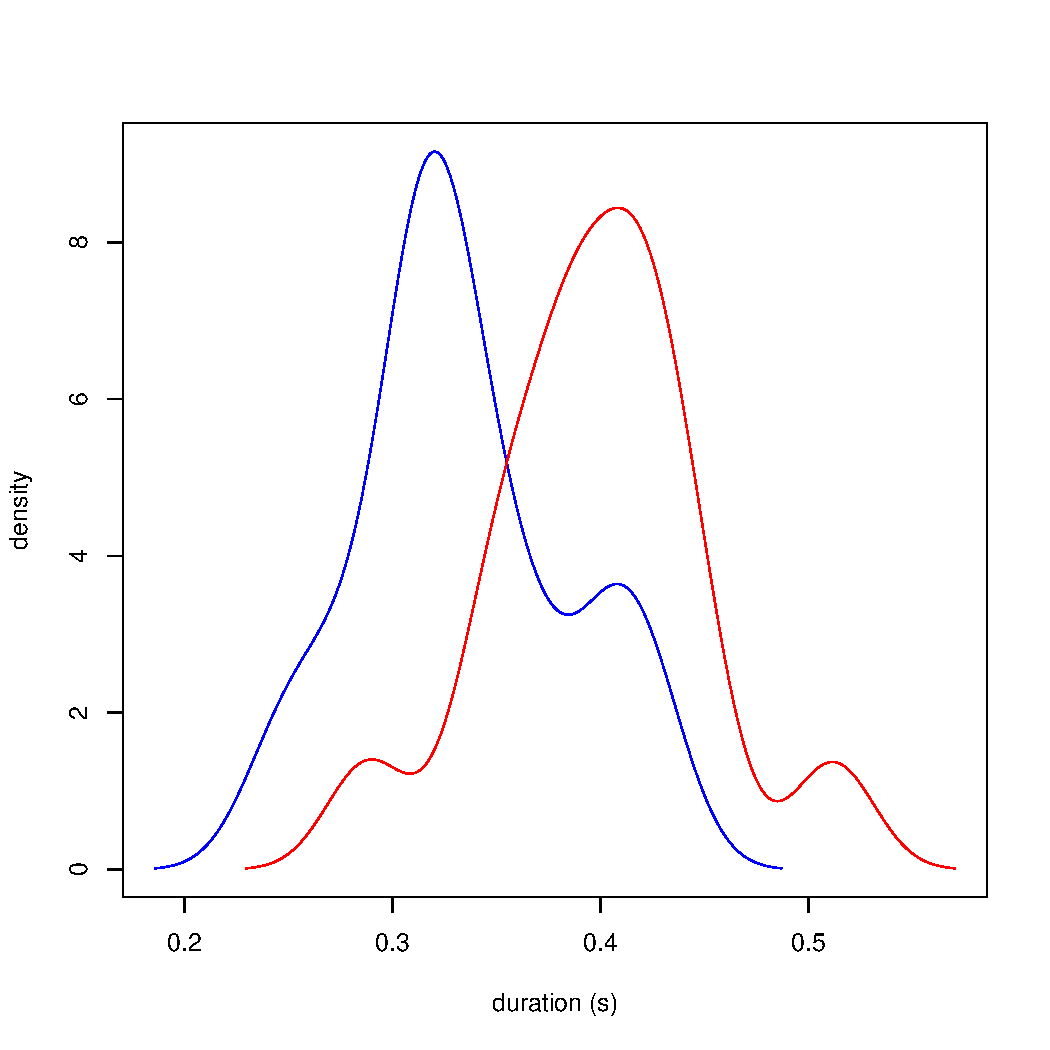
\includegraphics[width=\maxwidth]{img/bi-rho-dens-1} 

\end{knitrout}

\begin{knitrout}
\definecolor{shadecolor}{rgb}{0.969, 0.969, 0.969}\color{fgcolor}\begin{kframe}
\begin{alltt}
\hlkwd{boxplot}\hlstd{(norm_vowel} \hlopt{~} \hlstd{asp,}
        \hlkwc{data} \hlstd{= di_rho,}
        \hlkwc{names} \hlstd{=} \hlkwd{c}\hlstd{(}\hlstr{"non-asp"}\hlstd{,} \hlstr{"asp"}\hlstd{),}
        \hlkwc{ylab} \hlstd{=} \hlstr{"duration (s)"}\hlstd{,}
        \hlkwc{main} \hlstd{=} \hlstr{"Duration (in seconds) of modal voicing in CVRCV words"}
        \hlstd{)}
\end{alltt}
\end{kframe}
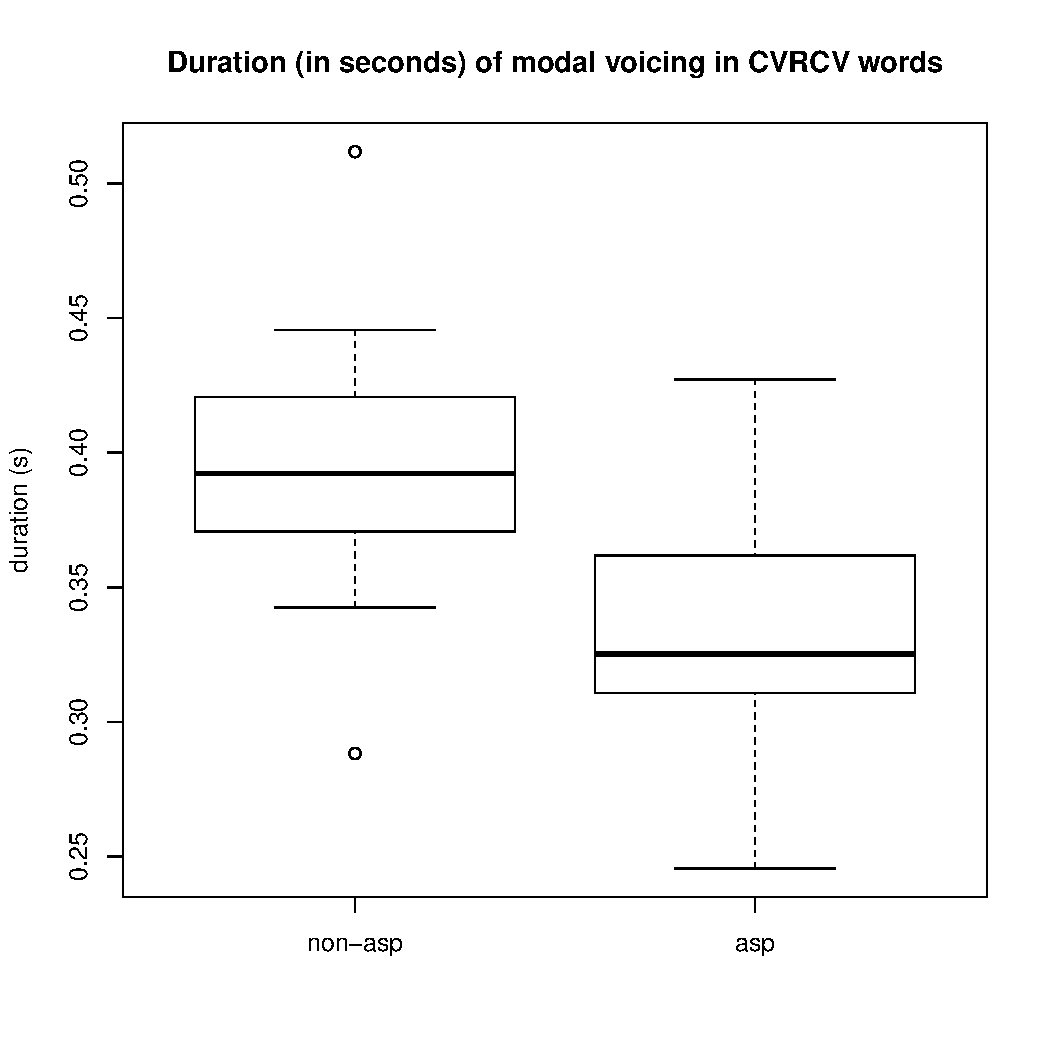
\includegraphics[width=\maxwidth]{img/bi-rho-box-1} 

\end{knitrout}

\begin{knitrout}
\definecolor{shadecolor}{rgb}{0.969, 0.969, 0.969}\color{fgcolor}\begin{kframe}
\begin{alltt}
\hlkwd{shapiro.test}\hlstd{(di_rho_asp)}
\end{alltt}
\begin{verbatim}
## 
## 	Shapiro-Wilk normality test
## 
## data:  di_rho_asp
## W = 0.96487, p-value = 0.7762
\end{verbatim}
\begin{alltt}
\hlkwd{shapiro.test}\hlstd{(di_rho_nasp)}
\end{alltt}
\begin{verbatim}
## 
## 	Shapiro-Wilk normality test
## 
## data:  di_rho_nasp
## W = 0.97208, p-value = 0.8876
\end{verbatim}
\begin{alltt}
\hlkwd{t.test}\hlstd{(norm_vowel} \hlopt{~} \hlstd{asp,} \hlkwc{data} \hlstd{= di_rho)}
\end{alltt}
\begin{verbatim}
## 
## 	Welch Two Sample t-test
## 
## data:  norm_vowel by asp
## t = 3.4013, df = 27.988, p-value = 0.002036
## alternative hypothesis: true difference in means is not equal to 0
## 95 percent confidence interval:
##  0.02544551 0.10250100
## sample estimates:
##  mean in group no mean in group yes 
##         0.3982628         0.3342896
\end{verbatim}
\end{kframe}
\end{knitrout}

As with monosyllabic words, we should check if the duration of bisyllabic words is affected by the presence vs. absence of preaspiration.

\begin{knitrout}
\definecolor{shadecolor}{rgb}{0.969, 0.969, 0.969}\color{fgcolor}\begin{kframe}
\begin{alltt}
\hlkwd{boxplot}\hlstd{(dur_word} \hlopt{~} \hlstd{asp,} \hlkwc{data} \hlstd{= bi)}
\end{alltt}
\end{kframe}
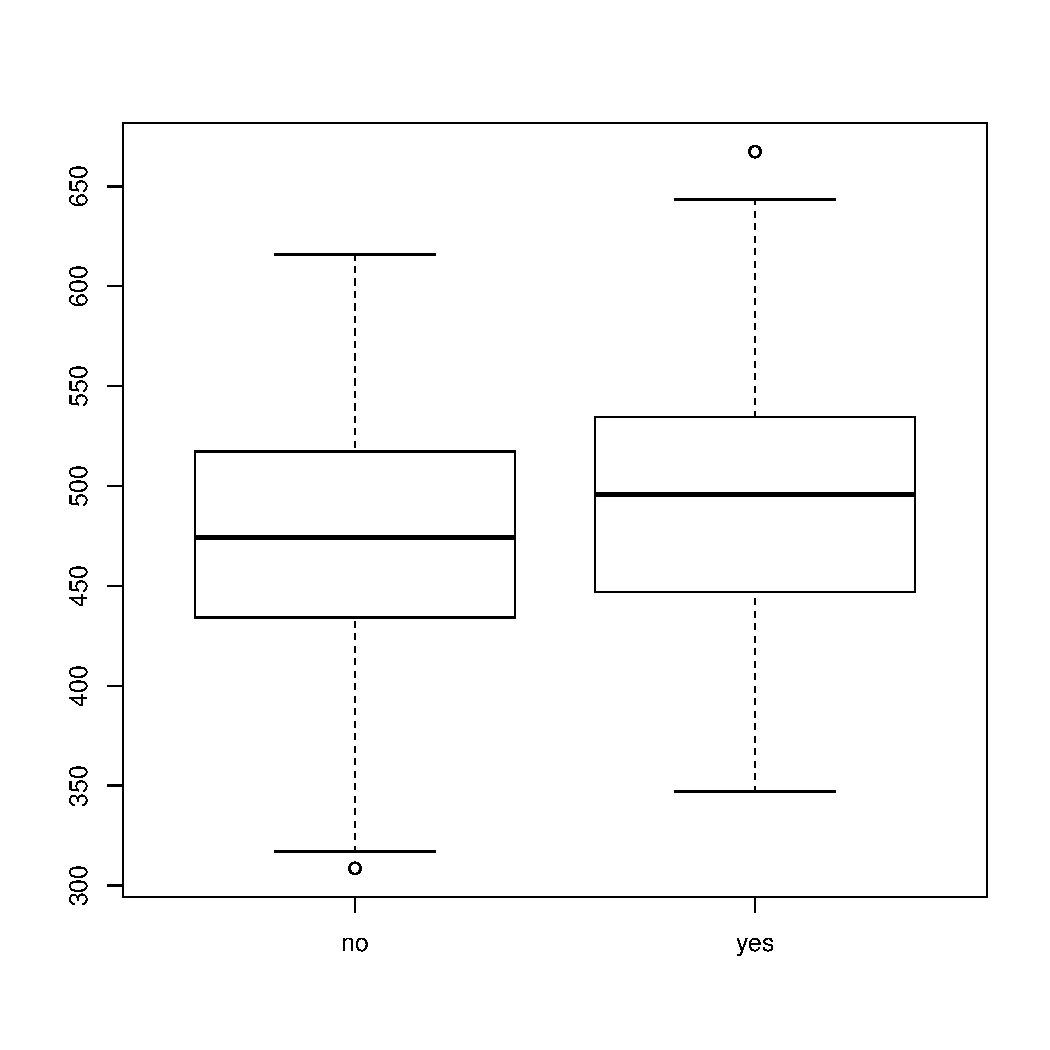
\includegraphics[width=\maxwidth]{img/bi-box-1} 

\end{knitrout}

\begin{knitrout}
\definecolor{shadecolor}{rgb}{0.969, 0.969, 0.969}\color{fgcolor}\begin{kframe}
\begin{alltt}
\hlkwd{shapiro.test}\hlstd{(bi}\hlopt{$}\hlstd{dur_word[bi}\hlopt{$}\hlstd{asp} \hlopt{==} \hlstr{"yes"}\hlstd{])}
\end{alltt}
\begin{verbatim}
## 
## 	Shapiro-Wilk normality test
## 
## data:  bi$dur_word[bi$asp == "yes"]
## W = 0.9923, p-value = 0.4437
\end{verbatim}
\begin{alltt}
\hlkwd{shapiro.test}\hlstd{(bi}\hlopt{$}\hlstd{dur_word[bi}\hlopt{$}\hlstd{asp} \hlopt{==} \hlstr{"no"}\hlstd{])}
\end{alltt}
\begin{verbatim}
## 
## 	Shapiro-Wilk normality test
## 
## data:  bi$dur_word[bi$asp == "no"]
## W = 0.98318, p-value = 0.008744
\end{verbatim}
\end{kframe}
\end{knitrout}

\begin{knitrout}
\definecolor{shadecolor}{rgb}{0.969, 0.969, 0.969}\color{fgcolor}\begin{kframe}
\begin{alltt}
\hlkwd{wilcox.test}\hlstd{(dur_word} \hlopt{~} \hlstd{asp,} \hlkwc{data} \hlstd{= bi)}
\end{alltt}
\begin{verbatim}
## 
## 	Wilcoxon rank sum test with continuity correction
## 
## data:  dur_word by asp
## W = 17319, p-value = 0.004711
## alternative hypothesis: true location shift is not equal to 0
\end{verbatim}
\end{kframe}
\end{knitrout}

According to a Wilcoxon-test, the duration of bisyllabic words is affected by the presence vs. absence of preaspiration.


\begin{knitrout}
\definecolor{shadecolor}{rgb}{0.969, 0.969, 0.969}\color{fgcolor}\begin{kframe}
\begin{alltt}
\hlkwd{boxplot}\hlstd{(dur_word} \hlopt{~} \hlstd{asp,} \hlkwc{data} \hlstd{= results)}
\end{alltt}
\end{kframe}
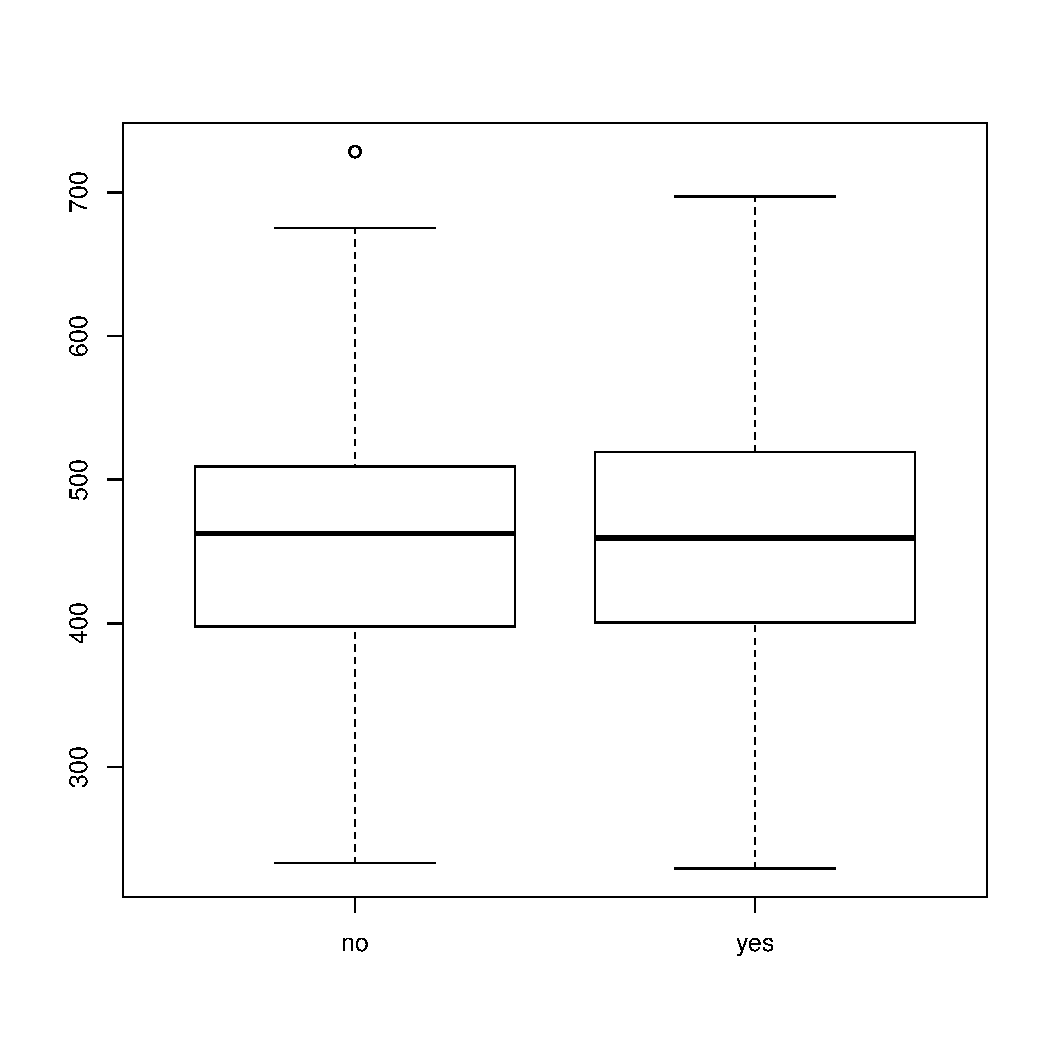
\includegraphics[width=\maxwidth]{img/results-box-1} 

\end{knitrout}

\begin{knitrout}
\definecolor{shadecolor}{rgb}{0.969, 0.969, 0.969}\color{fgcolor}\begin{kframe}
\begin{alltt}
\hlkwd{shapiro.test}\hlstd{(results}\hlopt{$}\hlstd{dur_word[results}\hlopt{$}\hlstd{asp} \hlopt{==} \hlstr{"yes"}\hlstd{])}
\end{alltt}
\begin{verbatim}
## 
## 	Shapiro-Wilk normality test
## 
## data:  results$dur_word[results$asp == "yes"]
## W = 0.99506, p-value = 0.2236
\end{verbatim}
\begin{alltt}
\hlkwd{shapiro.test}\hlstd{(results}\hlopt{$}\hlstd{dur_word[results}\hlopt{$}\hlstd{asp} \hlopt{==} \hlstr{"no"}\hlstd{])}
\end{alltt}
\begin{verbatim}
## 
## 	Shapiro-Wilk normality test
## 
## data:  results$dur_word[results$asp == "no"]
## W = 0.99183, p-value = 0.02449
\end{verbatim}
\end{kframe}
\end{knitrout}

\begin{knitrout}
\definecolor{shadecolor}{rgb}{0.969, 0.969, 0.969}\color{fgcolor}\begin{kframe}
\begin{alltt}
\hlkwd{wilcox.test}\hlstd{(dur_word} \hlopt{~} \hlstd{asp,} \hlkwc{data} \hlstd{= results)}
\end{alltt}
\begin{verbatim}
## 
## 	Wilcoxon rank sum test with continuity correction
## 
## data:  dur_word by asp
## W = 79555, p-value = 0.3918
## alternative hypothesis: true location shift is not equal to 0
\end{verbatim}
\end{kframe}
\end{knitrout}

\section{VOR}
\begin{knitrout}
\definecolor{shadecolor}{rgb}{0.969, 0.969, 0.969}\color{fgcolor}\begin{kframe}
\begin{alltt}
\hlkwd{boxplot}\hlstd{(vor} \hlopt{~} \hlstd{asp,} \hlkwc{data} \hlstd{= results)}
\end{alltt}
\end{kframe}
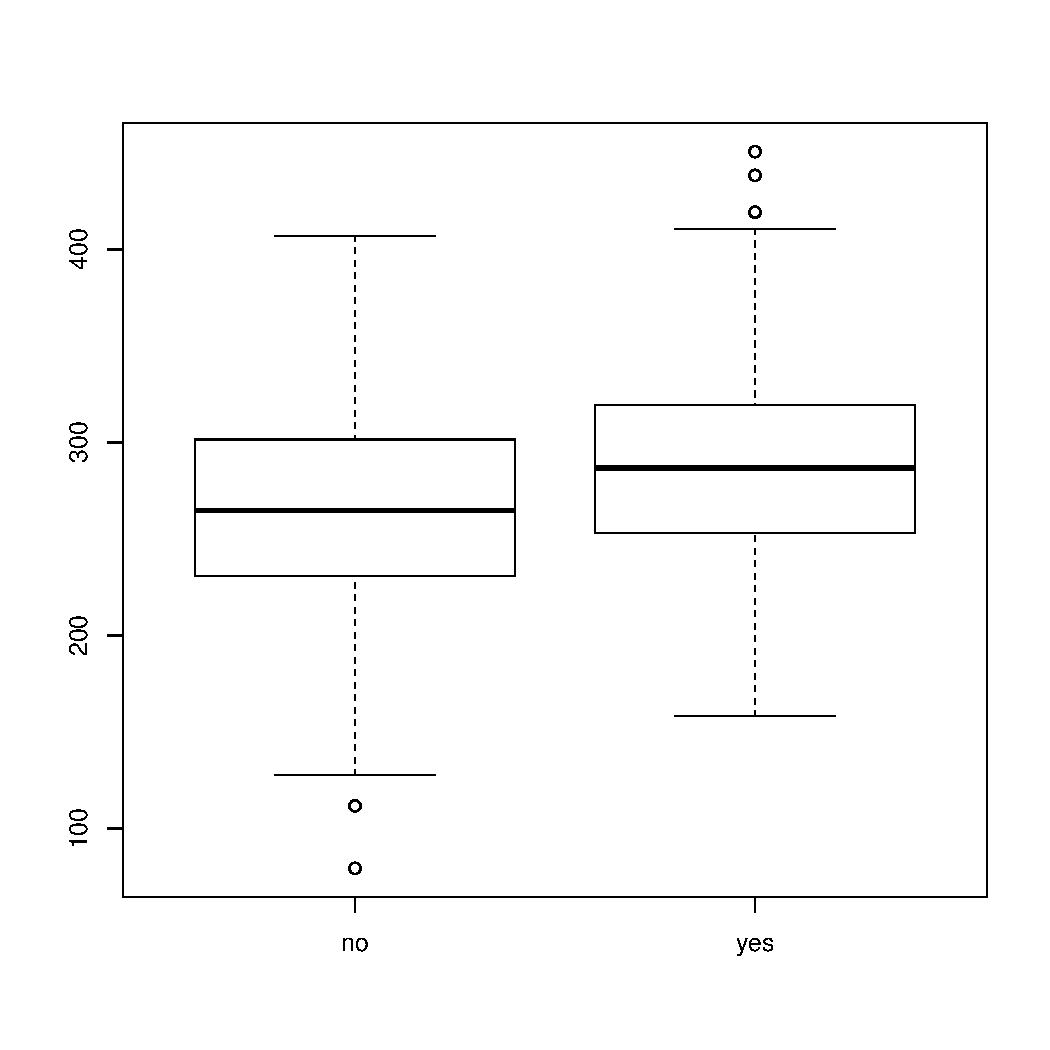
\includegraphics[width=\maxwidth]{img/unnamed-chunk-22-1} 
\begin{kframe}\begin{alltt}
\hlkwd{shapiro.test}\hlstd{(results}\hlopt{$}\hlstd{vor[results}\hlopt{$}\hlstd{asp} \hlopt{==} \hlstr{"yes"}\hlstd{])}
\end{alltt}
\begin{verbatim}
## 
## 	Shapiro-Wilk normality test
## 
## data:  results$vor[results$asp == "yes"]
## W = 0.9958, p-value = 0.3577
\end{verbatim}
\begin{alltt}
\hlkwd{shapiro.test}\hlstd{(results}\hlopt{$}\hlstd{vor[results}\hlopt{$}\hlstd{asp} \hlopt{==} \hlstr{"no"}\hlstd{])}
\end{alltt}
\begin{verbatim}
## 
## 	Shapiro-Wilk normality test
## 
## data:  results$vor[results$asp == "no"]
## W = 0.99719, p-value = 0.7422
\end{verbatim}
\begin{alltt}
\hlkwd{t.test}\hlstd{(vor} \hlopt{~} \hlstd{asp,} \hlkwc{data} \hlstd{= results)}
\end{alltt}
\begin{verbatim}
## 
## 	Welch Two Sample t-test
## 
## data:  vor by asp
## t = -6.1393, df = 790.14, p-value = 1.311e-09
## alternative hypothesis: true difference in means is not equal to 0
## 95 percent confidence interval:
##  -28.86452 -14.87835
## sample estimates:
##  mean in group no mean in group yes 
##          265.3115          287.1829
\end{verbatim}
\end{kframe}
\end{knitrout}

\section{Closure}
\begin{knitrout}
\definecolor{shadecolor}{rgb}{0.969, 0.969, 0.969}\color{fgcolor}\begin{kframe}
\begin{alltt}
\hlkwd{wilcox.test}\hlstd{(norm_clos} \hlopt{~} \hlstd{asp, mono_nas)}
\end{alltt}
\begin{verbatim}
## 
## 	Wilcoxon rank sum test
## 
## data:  norm_clos by asp
## W = 643, p-value = 0.2487
## alternative hypothesis: true location shift is not equal to 0
\end{verbatim}
\begin{alltt}
\hlkwd{wilcox.test}\hlstd{(norm_clos} \hlopt{~} \hlstd{asp, mono_lat)}
\end{alltt}
\begin{verbatim}
## 
## 	Wilcoxon rank sum test
## 
## data:  norm_clos by asp
## W = 122, p-value = 0.1257
## alternative hypothesis: true location shift is not equal to 0
\end{verbatim}
\begin{alltt}
\hlkwd{wilcox.test}\hlstd{(norm_clos} \hlopt{~} \hlstd{asp, di_nas)}
\end{alltt}
\begin{verbatim}
## 
## 	Wilcoxon rank sum test with continuity correction
## 
## data:  norm_clos by asp
## W = 1829, p-value = 0.9733
## alternative hypothesis: true location shift is not equal to 0
\end{verbatim}
\begin{alltt}
\hlkwd{wilcox.test}\hlstd{(norm_clos} \hlopt{~} \hlstd{asp, di_lat)}
\end{alltt}
\begin{verbatim}
## 
## 	Wilcoxon rank sum test
## 
## data:  norm_clos by asp
## W = 546, p-value = 0.02392
## alternative hypothesis: true location shift is not equal to 0
\end{verbatim}
\begin{alltt}
\hlkwd{wilcox.test}\hlstd{(norm_clos} \hlopt{~} \hlstd{asp, di_rho)}
\end{alltt}
\begin{verbatim}
## 
## 	Wilcoxon rank sum test
## 
## data:  norm_clos by asp
## W = 206, p-value = 2.655e-05
## alternative hypothesis: true location shift is not equal to 0
\end{verbatim}
\end{kframe}
\end{knitrout}

\section{Sonorant duration}
\begin{knitrout}
\definecolor{shadecolor}{rgb}{0.969, 0.969, 0.969}\color{fgcolor}\begin{kframe}
\begin{alltt}
\hlkwd{wilcox.test}\hlstd{(norm_mann} \hlopt{~} \hlstd{asp, mono_nas)}
\end{alltt}
\begin{verbatim}
## 
## 	Wilcoxon rank sum test
## 
## data:  norm_mann by asp
## W = 338, p-value = 0.006585
## alternative hypothesis: true location shift is not equal to 0
\end{verbatim}
\begin{alltt}
\hlkwd{wilcox.test}\hlstd{(norm_mann} \hlopt{~} \hlstd{asp, mono_lat)}
\end{alltt}
\begin{verbatim}
## 
## 	Wilcoxon rank sum test
## 
## data:  norm_mann by asp
## W = 25, p-value = 0.0009344
## alternative hypothesis: true location shift is not equal to 0
\end{verbatim}
\begin{alltt}
\hlkwd{wilcox.test}\hlstd{(norm_mann} \hlopt{~} \hlstd{asp, di_nas)}
\end{alltt}
\begin{verbatim}
## 
## 	Wilcoxon rank sum test with continuity correction
## 
## data:  norm_mann by asp
## W = 1190, p-value = 0.0008771
## alternative hypothesis: true location shift is not equal to 0
\end{verbatim}
\begin{alltt}
\hlkwd{wilcox.test}\hlstd{(norm_mann} \hlopt{~} \hlstd{asp, di_lat)}
\end{alltt}
\begin{verbatim}
## 
## 	Wilcoxon rank sum test
## 
## data:  norm_mann by asp
## W = 58, p-value = 6.607e-10
## alternative hypothesis: true location shift is not equal to 0
\end{verbatim}
\begin{alltt}
\hlkwd{wilcox.test}\hlstd{(norm_mann} \hlopt{~} \hlstd{asp, di_rho)}
\end{alltt}
\begin{verbatim}
## 
## 	Wilcoxon rank sum test
## 
## data:  norm_mann by asp
## W = 6, p-value = 3.868e-07
## alternative hypothesis: true location shift is not equal to 0
\end{verbatim}
\begin{alltt}
\hlkwd{boxplot}\hlstd{(dur_mann} \hlopt{~} \hlstd{asp, mono_nas)}
\end{alltt}
\end{kframe}
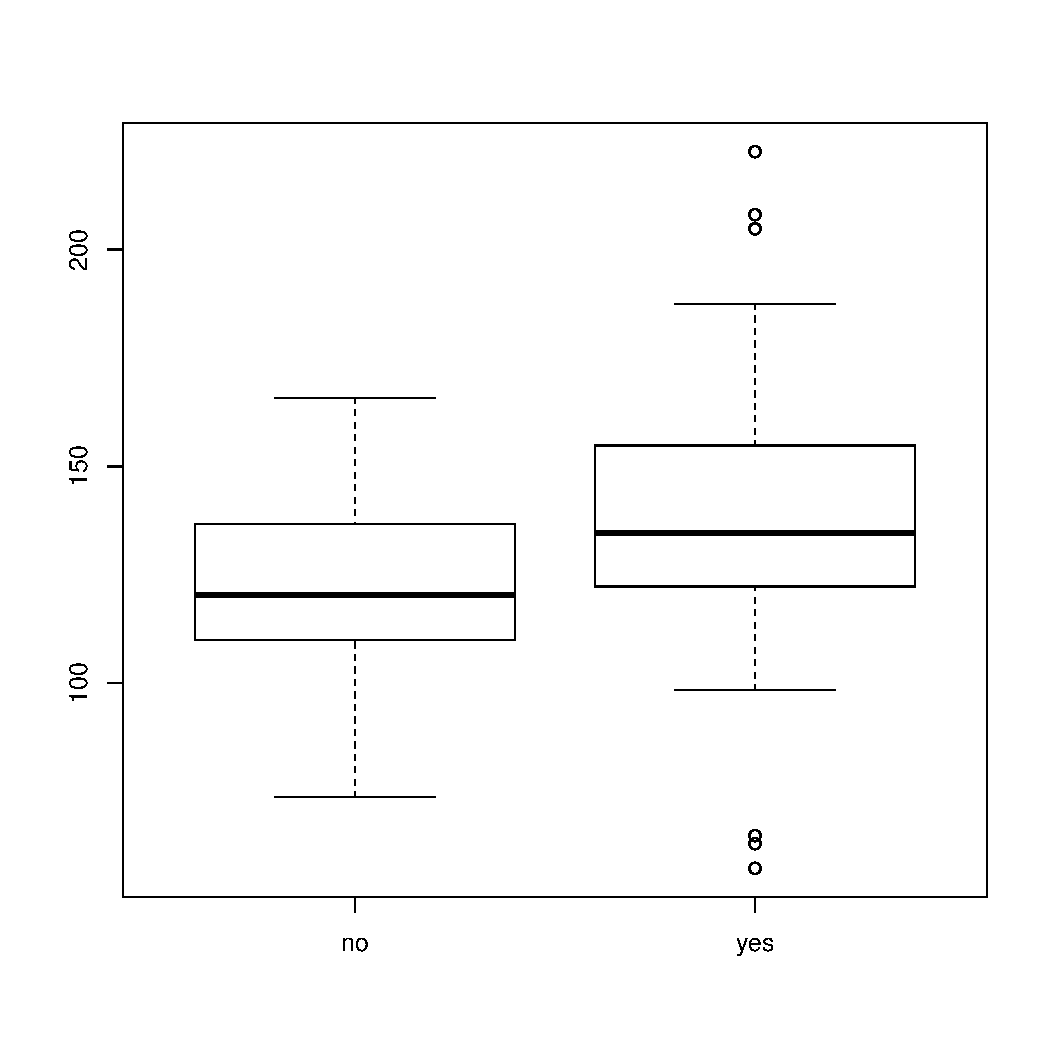
\includegraphics[width=\maxwidth]{img/unnamed-chunk-24-1} 
\begin{kframe}\begin{alltt}
\hlkwd{boxplot}\hlstd{(dur_mann} \hlopt{~} \hlstd{asp, mono_lat)}
\end{alltt}
\end{kframe}
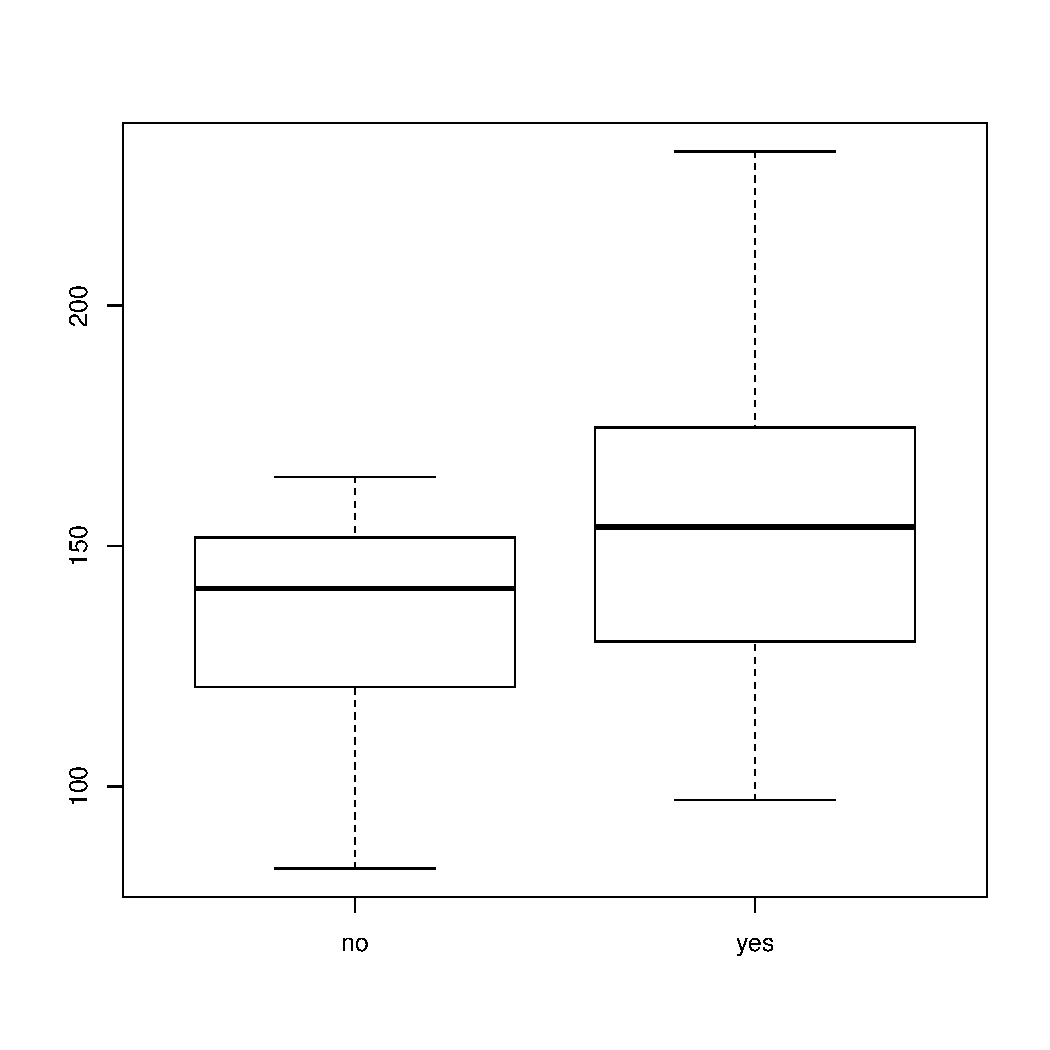
\includegraphics[width=\maxwidth]{img/unnamed-chunk-24-2} 
\begin{kframe}\begin{alltt}
\hlkwd{boxplot}\hlstd{(dur_mann} \hlopt{~} \hlstd{asp, di_nas)}
\end{alltt}
\end{kframe}
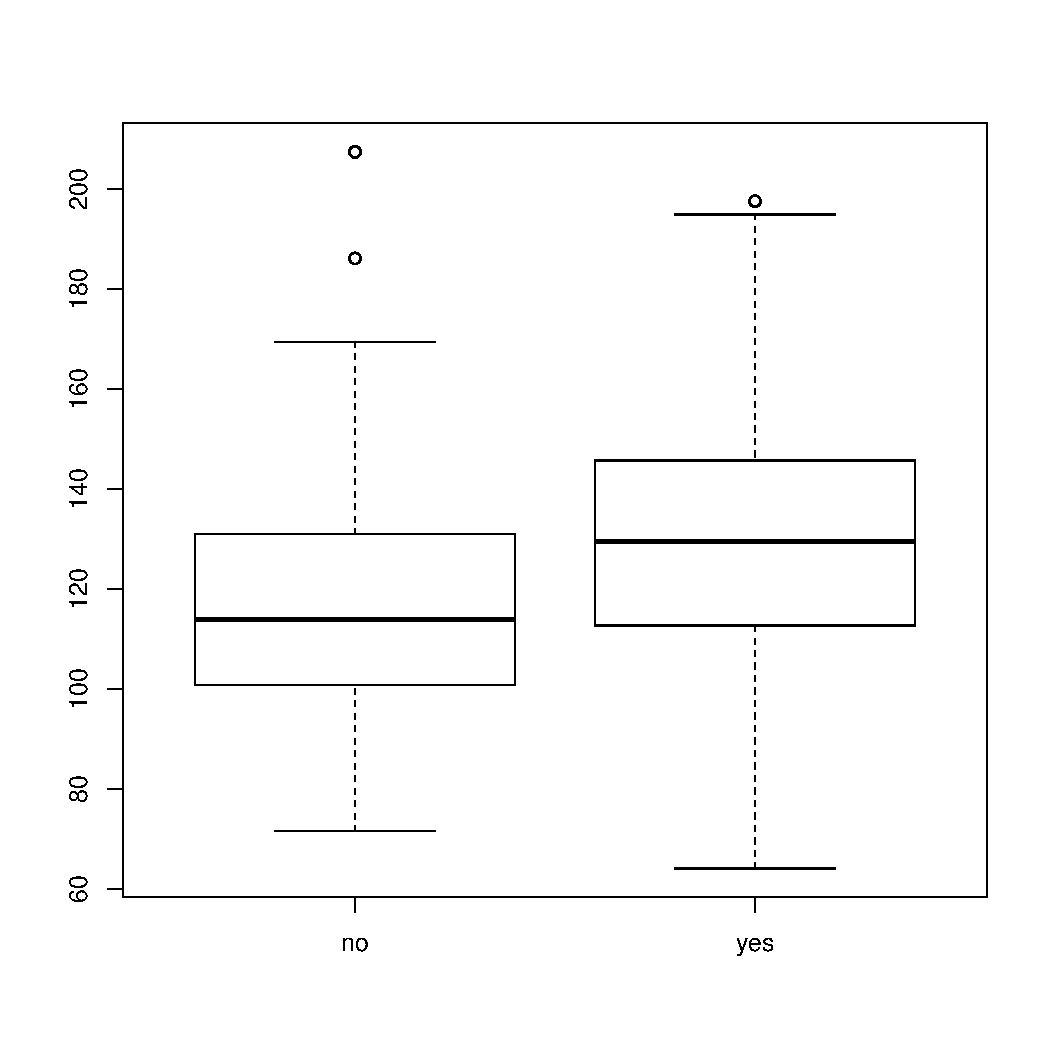
\includegraphics[width=\maxwidth]{img/unnamed-chunk-24-3} 
\begin{kframe}\begin{alltt}
\hlkwd{boxplot}\hlstd{(dur_mann} \hlopt{~} \hlstd{asp, di_lat)}
\end{alltt}
\end{kframe}
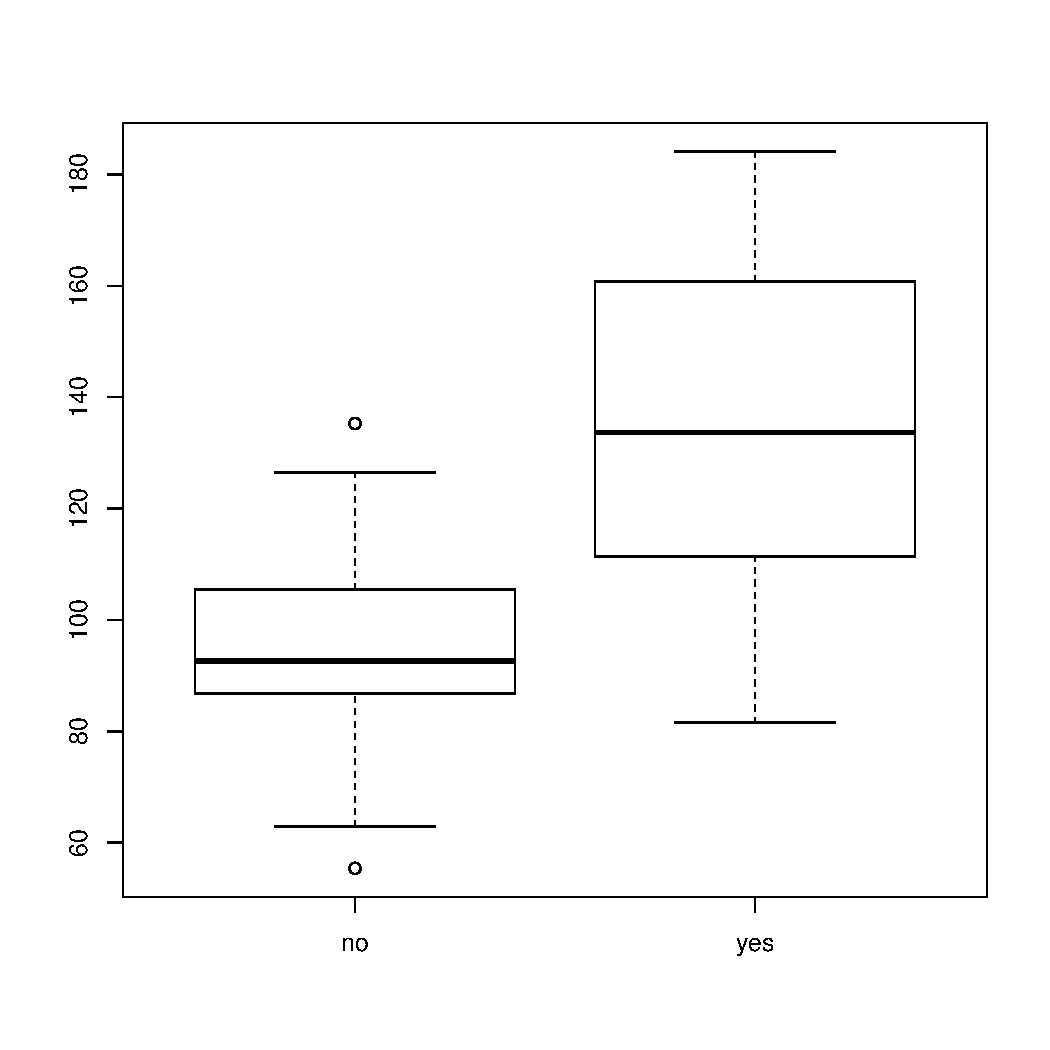
\includegraphics[width=\maxwidth]{img/unnamed-chunk-24-4} 
\begin{kframe}\begin{alltt}
\hlkwd{boxplot}\hlstd{(dur_mann} \hlopt{~} \hlstd{asp, di_rho)}
\end{alltt}
\end{kframe}
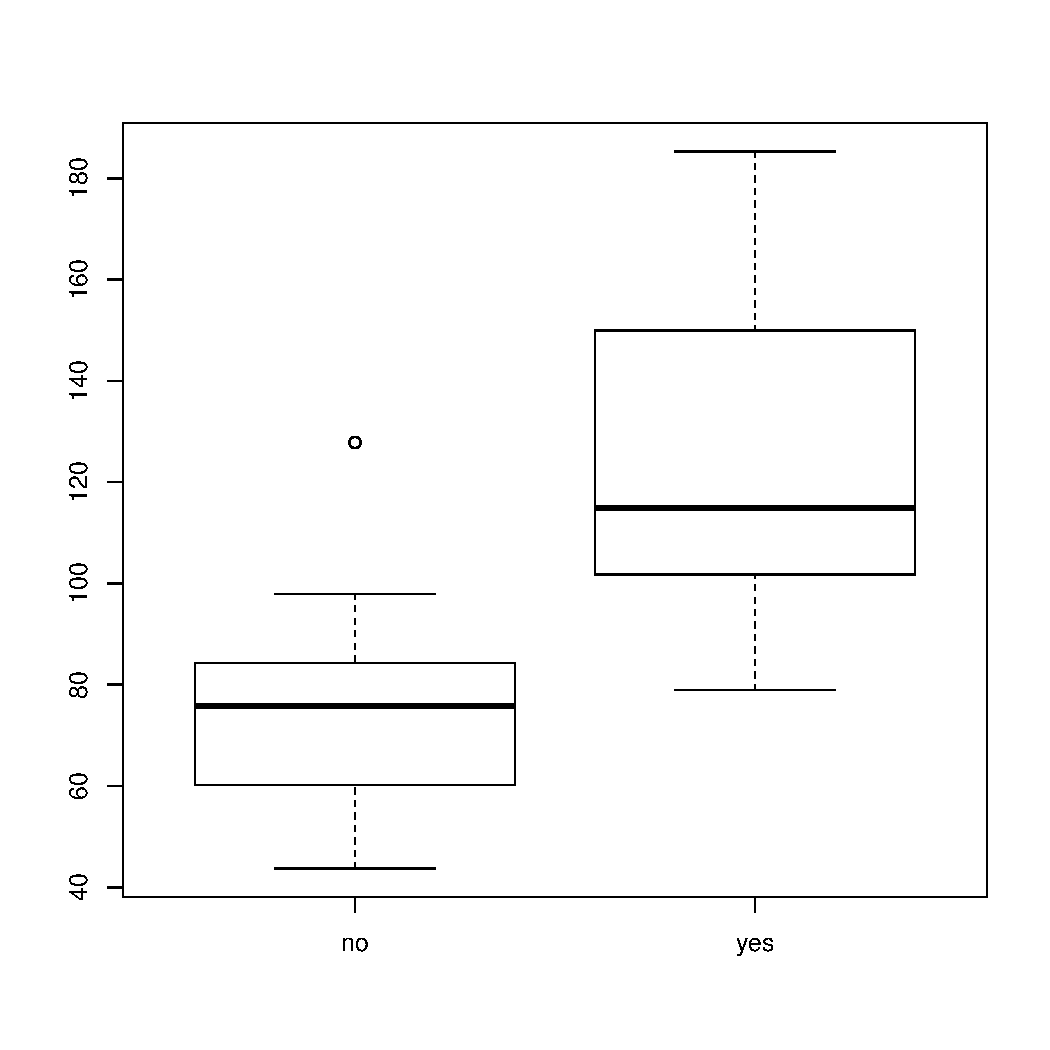
\includegraphics[width=\maxwidth]{img/unnamed-chunk-24-5} 

\end{knitrout}

\end{document}
